%%%%%%%%%%%%%%%%%%%%%%%%%%%%%%%%%%%%%%%%%%%%%%%%%%%%%%%%%%%%%%%%%%%%%%%%%%%%%%%%
%%%%%%%%%%%%%%%%%%%%%%%%%%%%%%%%%%%%%%%%%%%%%%%%%%%%%%%%%%%%%%%%%%%%%%%%%%%%%%%%
%%                                                                            %%
%% thesistemplate.tex version 4.10 (2025/06/30)                               %%
%% The LaTeX template file to be used with the aaltothesis.sty (version 4.10) %%
%% style file.                                                                %%
%% This package requires pdfx.sty v. 1.5.84 (2017/05/18) or newer.            %%
%%                                                                            %%
%% This is licensed under the terms of the MIT license below.                 %%
%%                                                                            %%
%% Written by Luis R.J. Costa.                                                %%
%% Currently developed at Teacher services, Learning Services of Aalto        %%
%% University by Luis R.J. Costa since May 2019.                              %%
%%                                                                            %%
%% Copyright 2017-2025 aaltothesis.cls by Luis R.J. Costa,                    %%
%% luis.costa@aalto.fi.                                                       %%
%% Copyright 2017-2018 Swedish translations in aaltothesis.cls by Elisabeth   %%
%% Nyberg and Henrik Wallén henrik.wallen@aalto.fi.                           %%
%% Copyright 2017-2018 Finnish documentation in the template opinnatepohja.tex%%
%% by Perttu Puska, perttu.puska@aalto.fi, and Luis R.J. Costa.               %%
%% Finnish documentation in the template opinnatepohja.tex translated from    %%
%% the English template documentation.                                        %%
%% Copyright 2025 English template thesistemplate.tex by Luis R.J. Costa,     %%
%% Maurice Forget, Henrik Wallén.                                             %%
%% Copyright 2018-2025 Swedish template kandidatarbetsbotten.tex by Henrik    %%
%% Wallen.                                                                    %%
%%                                                                            %%
%% Permission is hereby granted, free of charge, to any person obtaining a    %%
%% copy of this software and associated documentation files (the "Software"), %%
%% to deal in the Software without restriction, including without limitation  %%
%% the rights to use, copy, modify, merge, publish, distribute, sublicense,   %%
%% and/or sell copies of the Software, and to permit persons to whom the      %%
%% Software is furnished to do so, subject to the following conditions:       %%
%% The above copyright notice and this permission notice shall be included in %%
%% all copies or substantial portions of the Software.                        %%
%% THE SOFTWARE IS PROVIDED "AS IS", WITHOUT WARRANTY OF ANY KIND, EXPRESS OR %%
%% IMPLIED, INCLUDING BUT NOT LIMITED TO THE WARRANTIES OF MERCHANTABILITY,   %%
%% FITNESS FOR A PARTICULAR PURPOSE AND NONINFRINGEMENT. IN NO EVENT SHALL    %%
%% THE AUTHORS OR COPYRIGHT HOLDERS BE LIABLE FOR ANY CLAIM, DAMAGES OR OTHER %%
%% LIABILITY, WHETHER IN AN ACTION OF CONTRACT, TORT OR OTHERWISE, ARISING    %%
%% FROM, OUT OF OR IN CONNECTION WITH THE SOFTWARE OR THE USE OR OTHER        %%
%% DEALINGS IN THE SOFTWARE.                                                  %%
%%                                                                            %%
%%                                                                            %%
%%%%%%%%%%%%%%%%%%%%%%%%%%%%%%%%%%%%%%%%%%%%%%%%%%%%%%%%%%%%%%%%%%%%%%%%%%%%%%%%
%%                                                                            %%
%%                                                                            %%
%% An example for writting your thesis using LaTeX                            %%
%% Original version and development work by Luis Costa, changes to the text   %% 
%% in the Finnish template by Perttu Puska.                                   %%
%% Support for Swedish added 15092014                                         %%
%% PDF/A-b support added on 15092017                                          %%
%% PDF/A-2 support added on 24042018                                          %%
%% Layout design and typesettin changed 15072021                              %%
%%                                                                            %%
%% This example consists of the files                                         %%
%%       thesistemplate.tex (version 4.10) (for text in English)              %%
%%       opinnaytepohja.tex (version 4.10) (for text in Finnish)              %%
%%       kandidatarbetsbotten.tex (version 1.20) (for text in Swedish)        %%
%%       thesistemplate_short.tex (version 4.10) (abridged for text in        %%
%%                                                English)                    %%
%%       aaltothesis.cls (version 4.10)                                       %%
%%       linediagram.pdf (graphics file)                                      %%
%%       curves.pdf      (graphics file)                                      %%
%%       ledspole.jpg    (graphics file)                                      %%
%%                                                                            %%
%%                                                                            %%
%% Typeset in Linux with                                                      %%
%% pdflatex: (recommended method)                                             %%
%%             $ pdflatex thesistemplate                                      %%
%%             $ pdflatex thesistemplate                                      %%
%%                                                                            %%
%%   The result is the file thesistemplate.pdf that is PDF/A compliant, if    %%
%%   you have chosen the proper \documenclass options (see comments below)    %%
%%   and your included graphics files have no problems.                       %%
%%                                                                            %%
%%                                                                            %%
%% Explanatory comments in this example begin with the characters %%, and     %%
%% changes that the user can make with the character %                        %%
%%                                                                            %%
%%%%%%%%%%%%%%%%%%%%%%%%%%%%%%%%%%%%%%%%%%%%%%%%%%%%%%%%%%%%%%%%%%%%%%%%%%%%%%%%
%%%%%%%%%%%%%%%%%%%%%%%%%%%%%%%%%%%%%%%%%%%%%%%%%%%%%%%%%%%%%%%%%%%%%%%%%%%%%%%%
%%
%% WHAT is PDF/A
%%
%% PDF/A is the ISO-standardized version of the pdf. The standard's goal is to
%% ensure that he file is reproducable even after a long time. PDF/A differs
%% from pdf in that it allows only those pdf features that support long-term
%% archiving of a file. For example, PDF/A requires that all used fonts are
%% embedded in the file, whereas a normal pdf can contain only a link to the
%% fonts in the system of the reader of the file. PDF/A also requires, among
%% other things, data on colour definition and the encryption used.
%% Currently three PDF/A standards exist:
%% PDF/A-1: based on PDF 1.4, standard ISO19005-1, published in 2005.
%%          Includes all the requirements essential for long-term archiving.
%% PDF/A-2: based on PDF 1.7, standard ISO19005-2, published in 2011.
%%          In addition to the above, it supports embedding of OpenType fonts,
%%          transparency in the colour definition and digital signatures.
%% PDF/A-3: based on PDF 1.7, standard ISO19005-3, published in 2012.
%%          Differs from the above only in that it allows embedding of files in
%%          any format (e.g., xml, csv, cad, spreadsheet or wordprocessing
%%          formats) into the pdf file.
%% PDF/A-4: based on PDF 2.0, standard ISO19005-4, published in November 2020.
%%
%% PDF/A-1 files are not necessarily PDF/A-2 -compatible and PDF/A-2 are not
%% necessarily PDF/A-1 -compatible.
%% Standards PDF/A-1, PDF/A-2 and PDF/A-3 have two levels:
%% b: (basic) requires that the visual appearance of the document is reliably
%%    reproduceable.
%% a (accessible) in addition to the b-level requirements, specifies how
%%   accessible the pdf file is to assistive software, say, for the physically
%%   impaired.
%% The PDF/A-4 standard does not have additional levels like in the earlier
%% standards.
%% For more details on PDF/A, see, e.g., 
%% https://www.loc.gov/preservation/digital/formats/fdd/fdd000318.shtml or
%% https://www.pdfa.org/resource/iso-19005-pdfa/
%%
%%
%% WHICH PDF/A standard should my thesis conform to?
%%
%% Either to the PDF/A-2b or the PDF/A-1b standard. If all the figures and
%% graphs used in thesis work do not require transparency features, use either
%% PDF/A-1b or PFDF/A-2b. If you have figures with transparency
%% characteristics, use the PDF/A-2b standard. However, drawing applications
%% often use the transparency parameter, setting it to zero, to specify opacity
%% and get the basic 2-D visualisation. As a result, validation of PDF/A-1b
%% will fail. Use PDF/A-2b if PDF/A-1b validation fails.
%% Do not use the PDF/A-3b standard for your thesis.
%% The font to be used are specified in this templatenand they should not be
%% changed. In addition to not adhering to Aalto's visual guidelines, you may
%% have difficulties in producing a PDF/A-compliant PDF.
%%
%%
%% Validate your PDF/A file at https://www.pdf-online.com/osa/validate.aspx
%%
%%
%% WHAT graphics format can I use to produce my PDF/A compliant file?
%%
%% When using pdflatex to compile your work, favour the use of pdf, but you can
%% use the jpg or png format especially for photographs. You will have PDF/A 
%% compliance problems with figures in pdf if the fonts are not embedded in the
%% pdf file.
%% If you choose to use latex to compile your work, the only acceptable file
%% format for your figure is eps. DO NOT use the ps format for your figures.
%%
%% USE one of the following three \documentclass set-ups:
%% * the first when using pdflatex to directly typeset your document in the
%%   chosen pdf/a format for online publishing (centred page layout),
%% * the second for one-sided printing your thesis with the layout (wide left 
%%   margin), or
%% * the third for two-sided printing.
%%
\documentclass[english, 12pt, a4paper, elec, utf8, a-2b, online]{aaltothesis}
%\documentclass[english, 12pt, a4paper, elec, utf8, a-2b, print]{aaltothesis}
%\documentclass[english, 12pt, a4paper, elec, utf8, a-2b, print, twoside]{aaltothesis}

%% Use the following options in the \documentclass macro above:
%% your school: arts, biz, chem, elec, eng, sci
%% the character encoding scheme used by your editor: utf8, latin1
%% thesis language: english, finnish, swedish
%% make an archiveable PDF/A-1b or PDF/A-2b compliant file: a-1b, a-2b
%%                    (with pdflatex, a normal pdf containing metadata is
%%                     produced without the a-*b option)
%% typset for online document or print on paper: online, print
%%        online: typeset in symmetric layout and blue hypertext for online
%%                publishing
%%        print: typeset in a symmetric layout and black hypertext for printing
%%               on paper
%%          two-side printing: twoside (default is one-sided printing)
%%               typeset in a wide margin on the binding side of the page and
%%               black hypertext. Use with print only.
%%

%% Use one of these if you write in Finnish (or use the Finnish template
%% opinnaytepohja.tex)
%\documentclass[finnish, 12pt, a4paper, elec, utf8, a-1b, online]{aaltothesis}
%\documentclass[finnish, 12pt, a4paper, elec, utf8, a-1b, print]{aaltothesis}
%\documentclass[finnish, 12pt, a4paper, elec, utf8, a-1b, print, twoside]{aaltothesis}

%% Use one of these if you write in Swedish (or use the Swedish template
%% kandidatarbetsbotten.tex)
%\documentclass[swedish, 12pt, a4paper, elec, utf8, a-2b, online]{aaltothesis}
%\documentclass[swedish, 12pt, a4paper, elec, utf8, a-2b]{aaltothesis}
%\documentclass[swedish, 12pt, a4paper, elec, dvips, online]{aaltothesis}

%% FOR USERS OF AMS PACKAGES:
%% * newtxmath used in this template loads amsmath, so
%%   you needn't load it. If you want to use options in amsmath, load it here, 
%%   before \setupthesisfonts below to pass the options to amsmath.
%% * If you want to use amsthm, load it here before \setupthesisfonts to avoid
%%   a clash with newtxmath.
%% * If using amsmath with options and you want to use amsthm, load amsthms
%%   after amsmath, as described in the amsthm documentation.
%% * Don't use amsbsym or amsfonts. The symbols [and macros] there are defined in
%%   newtxmath and so clash if used.
%\usepackage[options]{amsmath}
%\usepackage{amsthm}

%% DO NOT MOVE OR REMOVE \setupthesisfonts
\setupthesisfonts

%%
%% Add here the packges you need
%%
\usepackage{graphicx}


%% For tables that span multiple pages; used to split a paraphrasing example in
%% the appendix. If you don't need it, remove it.
\usepackage{longtable}

\usepackage{pgfplots}

%% A package for generating Creative Commons copyright terms. If you don't use
%% the CC copyright terms, remove it, since otherwise undesired information may
%% be added to this document's metadata.
\usepackage[type={CC}, modifier={by-nc-sa}, version={4.0}]{doclicense}
%% Find below three examples for typesetting the CC license notice.

\usepackage[
backend=biber,
style=numeric-comp, % citations and references are numerical (Vancouver, IEEE)
sorting=none, % cited reference is first in the bibliography followed by all 
              % references in the database references.bib
firstinits=true, % show initial of first name in bibliography
urldate=long % date is expressed as Month dd, yyyy
]{biblatex}
\addbibresource{thesisreferences.bib}

%% Edit to conform to your degree programme
%% Capitalise the words in the name of the degree programme: it's a name
\degreeprogram{Computer, Communication and Information Sciences}
%%

%% Your major
%%
\major{Communications Engineering}
%%

%% Choose one of the three below
%%
%\univdegree{BSc}
\univdegree{MSc}
%\univdegree{Lic}
%%

%% Your name (self explanatory...)
%%
\thesisauthor{David Enberg}
%%

%% Your thesis title and possible subtitle comes here and possibly, again,
%% together with the Finnish or Swedish abstract. Do not hyphenate the title
%% (and subtitle), and avoid writing too long a title. Should LaTeX typeset a
%% long title (and/or subtitle) unsatisfactorily, you might have to force a
%% linebreak using the \\ control characters. In this case...
%% * Remember, the title should not be hyphenated!
%% * A possible 'and' in the title should not be the last word in the line; it
%%   begins the next line.
%% * Specify the title (and/or subtitle) again without the linebreak characters
%%   in the optional argument in box brackets. This is done because the title
%%   is part of the metadata in the pdf/a file, and the metadata cannot contain
%%   linebreaks.
%%
\thesistitle{Performance and interoperability of Server Message Block implementations over QUIC}
%\thesistitle[Title of the thesis]{Title of\\ the thesis}
%%
%% Either remove or leave \thesissubtitle{} empty if you don't use it
%%
\thesissubtitle{}
%\thesissubtitle[Subtitle of the thesis]{Subtitle of\\ the thesis}
%\thesissubtitle{}

%%
\place{Helsinki}
%%

%% The date for the bachelor's thesis is the day it is presented
%%
\date{5 November 2025}
%%

%% Thesis supervisor
%% Note the "\" character in the title after the period and before the space
%% and the following character string.
%% This is because the period is not the end of a sentence after which a
%% slightly longer space follows, but what is desired is a regular interword
%% space.
%%
\supervisor{PhD Pasi Sarolahti}
%%

%% Advisor(s)---two at the most---of the thesis. Check with your supervisor how
%% many official advisors you can have.
%%
\advisor{Bastian Shajit (MSc)}
%%

%% If you do your thesis work in a company of other institute, give the name of
%% the company or instution here. Otherwise, leave the macro empty, comment it
%% out, or remove it. This will remove this field from the abstract page.
%%
\collaborativepartner{Tuxera Oy}
%%

%% Aaltologo: syntax:
%% \uselogo{?|!|'|aalto?|aalto!|aalto'|<empty>}
%% The logo language is set to be the same as the thesis language.
%%
%\uselogo{?}
%\uselogo{!}
\uselogo{'}
%\uselogo{aalto?}
%\uselogo{aalto!}
%\uselogo{aalto'}
%\uselogo{}
%%

%%%%%%%%%%%%%%%%%%               COPYRIGHT TEXT               %%%%%%%%%%%%%%%%%%
%%%%%%%%%%%%%%%%%%%%%%%%%%%%%%%%%%%%%%%%%%%%%%%%%%%%%%%%%%%%%%%%%%%%%%%%%%%%%%%%

%% Copyright of a work is with the creator/author of the work regardless of
%% whether the copyright mark is explicitly in the work or not. You may, if you
%% wish---we encourage you to do so---publish your work under a Creative
%% Commons license (see creativecommons.org), in which case the license text
%% must be visible in the work. Write here the copyright text you want using the
%% macro \copyrighttext, which writes the text into the metadata of the pdf file
%% as well.
%%
%% Syntax:
%% \copyrigthtext{metadata text}{text visible on the page}
%%
%% CHOOSE ONE OF THE COPYRIGHT NOTICE STYLES BELOW.
%% IF USING THE CC TERMS, CHOOSE THE LICENSE YOU WANT TO USE.
%% The different CC licenses are listed at 
%% https://creativecommons.org/about/cclicenses/.
%% If you use the icons from the doclicense.sty package, add the package above
%% (\usepackage{doclicense}).
%% IMPORTANT NOTE!! Manually write the CC text in the \copyrighttext metadata
%% text field.
%%
%% NOTE: In the macros below, the text written in the metadata must have a
%% \noexpand macro before the \copyright special character. When not in pdf/a
%% mode (i.e. a-1b or a-2b are not specified in \documentclass), two \noexpands
%% are required in the metadata text to correctly render the copyright mark in
%% the pdf metadata. In pdf/a mode one \noexpand suffices.
%%
%% EXAMPLE OF PLAIN COPYRIGHT TEXT
%% The macros \copyright and \year below must be separated by the \ character 
%% (space chacter) from the text that follows. The macros in the argument of the
%% \copyrighttext macro automatically insert the year and the author's name.
%% (Note! \ThesisAuthor is an internal macro of the aaltothesis.cls class file).
%%
%\copyrighttext{Copyright \noexpand\textcopyright\ \number\year\ \ThesisAuthor}
%{Copyright \textcopyright{} \number\year{} \ThesisAuthor}
%%
%% Of course, the same text could have simply been written as
%% \copyrighttext{Copyright \noexpand\copyright\ 2018 Eddie Engineer}
%% {Copyright \copyright{} 2022 Eddie Engineer}
%%
%% EXAMPLES OF CC LICENSE: different ways to display the same license
%% 1. A simple Creative Commons license text with a link to the copyright notice:
%\copyrighttext{\noexpand\textcopyright\ \number\year. This work is 
%	licensed under a CC BY-NC-SA 4.0 license.}{\textcopyright{} 
%	\number\year. This work is licensed under a 
%	\href{https://creativecommons.org/licenses/by-nc-nd/4.0/}{CC BY-NC-SA 4.0} 
%	license.}
%
%% To get the URL of the license of your choice, go to 
%% https://creativecommons.org/about/cclicenses/, click on the chosen license
%% you want to use, and copy-and-paste the URL in the macro \href above.
%%
%% 2. A short Creative Commons license text containing the respective CC icons
%% (requires the package doclicense.sty to be added in the preamble as done
%% above) and a link to the corresponding Creative Commons license webpage (see
%% the doclicense package documentation for other license icons):
%\copyrighttext{\noexpand\textcopyright\ \number\year. This work is licensed
%	under a CC BY-NC-SA 4.0 license.}{
%	\parbox{95mm}{\noindent\textcopyright\ \number\year. \doclicenseText} 
%	\hspace{1em}\parbox{35mm}{\doclicenseImage}
%}
%%
%% 3. An expanded Creative Commons license text containing the respective CC
%% icons text and as generated by the doclicense.sty package (the license is set
%% via package options in \usepackage[options]{doclicense} above; see the
%% doclicense package documentation for other license texts and icons):
\copyrighttext{\noexpand\textcopyright\ \number\year. This work is 
	licensed under a Creative Commons "Attribution-NonCommercial-ShareAlike 4.0 
	International" (BY-NC-SA 4.0) license.}{\noindent\textcopyright\ \number
	\year \ \doclicenseThis}
%%%%%%%%%%%%%%%%%%%%%%%%%%%%%%%%%%%%%%%%%%%%%%%%%%%%%%%%%%%%%%%%%%%%%%%%%%%%%%%%


%% The English abstract:
%% All the details (name, title, etc.) on the abstract page appear as specified
%% above.
%% Thesis keywords:
%% Note! The keywords are separated using the \spc macro
%%
\keywords{QUIC\spc Server Message Block\spc MsQuic\spc Linux}
%%

%% The abstract text. This text in one paragraph is included in the metadata of
%% the pdf file as well as the abstract page. To have paragraphs in your
%% abstract rewrite it in the abstarct environment as described below.
%%
\thesisabstract{%
}

%% You can prevent LaTeX from writing into the xmpdata file (it contains all the 
%% metadata to be written into the pdf file) by setting the writexmpdata switch
%% to 'false'. This allows you to write the metadata in the correct format
%% directly into the file thesistemplate.xmpdata.
%\setboolean{writexmpdatafile}{false}


%% All that is printed on paper starts here
%%
\begin{document}

%% Create the coverpage
%%
\makecoverpage

%% Typeset the copyright text.
%% If you wish, you may leave out the copyright text from the human-readable
%% page of the pdf file. This may seem like a attractive idea for the printed
%% document especially if "Copyright (c) yyyy Eddie Engineer" is the only text
%% on the page. However, the recommendation is to print this copyright text.
%%
\makecopyrightpage

\clearpage
%% Note that when writing your thesis in English, place the English abstract
%% first followed by the possible Finnish or Swedish abstract.

%% Abstract text
%% All the details (name, title, etc.) on the abstract page appear as specified
%% above. Add your abstarct text with paragraphs here to have paragraphs in the
%% visible abstract page. Nonetheless, write the abstarct text without
%% paragraphs in the macro \thesismacro so that it is added to the metadata as
%% well.
%%
\begin{abstractpage}[english]
	The Server Message Block (SMB) protocol, a widely adopted protocol for network
	file sharing, traditionally relies upon TCP, which faces limitations in modern
	networking environments. The QUIC protocol offers a modern alternative, allowing
	for a secure, reliable transport with native multiplexing capabilities. The SMB
	protocol has added support for QUIC, but performance analysis of its impact and
	of protocol implementations outside of Windows is limited.

	In this thesis a QUIC transport layer for the Fusion SMB server was designed,
	implemented and evaluated in the Linux user space. A prototype was
	developed by integrating Microsoft's MsQuic library for QUIC capabilities. The
	thesis discusses the design of the transport layer and the architectural decisions
	made to interface with the existing server. The interoperability and performance of
	the implementation were benchmarked against
    Microsoft's implementation of SMB over QUIC in several different
	benchmarking scenarios. These results were compared to the performance of the standard
	encrypted TCP transport. The thesis concludes by discussing the performance
	results obtained, along with providing insights into the potential of leveraging
	advanced QUIC features in the SMB protocol, gained during the development process.
\end{abstractpage}

%% The text in the \thesisabstract macro is stored in the macro \abstractext, so
%% you can use the text metadata abstract directly as follows:
%%
%\begin{abstractpage}[english]
%	\abstracttext{}
%\end{abstractpage}


%% Force new page so that the Swedish abstract starts from a new page
\newpage

%% Swedish abstract. Delete it if you don't need it. 
%% 
%% Respecify those fields that differ from the earlier specification or simply
%% respecify all fields.
\thesistitle{Prestandautvärdering och interoperabilitet av SMB över QUIC lösningar}
\supervisor{FD Pasi Sarolahti}
\advisor{Bastian Shajit (MSc)}
\degreeprogram{Datakommunikationsteknik}
\collaborativepartner{Tuxera Ab}
%\date{30.6.2025}
%% Abstract keywords
\keywords{QUIC\spc Server Message Block\spc MsQuic\spc Linux}
%% Abstract text
\begin{abstractpage}[swedish]
	Server Message Block-protokollet (SMB), ett väletablerat protokoll för
	delning av filer över ett nätverk. Traditionellt förlitar sig SMB-protokollet
	på TCP, som medför begränsningar i moderna nätverksmiljöer. QUIC-protokollet
	erbjuder ett modernt alternativ som möjliggör säkert och tillförlitlig
	transport av information med inbyggt stöd för multiplexering. SMB-protokollet
	har utvidgats för att stöda QUIC, men prestandautvärderingar och implementeringar
	utanför Windows är begränsade.

	I detta examensarbete har ett QUIC-transportlager för Fusion SMB servern designats,
	implementerats och utvärderas i Linux användarrymd. En prototyp har utvecklas genom
	att integrera Microsofts MsQuic bibliotek, som erbjuder stöd för QUIC funktionalitet.
	Examensarbetet diskuterar designen av transportlagret och de beslut som tagits
	ur ett arkitekturperspektiv, för att samverka med den existerande servern. Implementationens
	prestanda och interoperabilitet jämfördes mot Microsofts implementation av SMB över QUIC,
	genom ett flertal test scenarion. Resultaten jämfördes med referensvärden från
	standardtransporten med krypterad TCP. Examensarbetet avslutas med en diskussion
	angående resultaten, samt ger insikter till potentialen att bättre utnyttja de avancerade
	QUIC funktionerna i SMB-protokollet, med hjälp av insikter som erhållits under
	utvecklingsprocessen.
\end{abstractpage}


\dothesispagenumbering{}

%% Preface
%%
%% This section is optional. Remove it if you do not want a preface.
\mysection{Preface}
%\mysection{Esipuhe}



\vspace{5cm}
Helsinki, 5 November 2025\\

\vspace{5mm}
{\hfill David C.\ Enberg \hspace{1cm}}

%% Force a new page after the preface
%%
\newpage


%% Table of contents. 
%%
\thesistableofcontents


%% Symbols and abbreviations
\mysection{Abbreviations}

\begin{tabular}{ll}
ACK & Acknowledgment \\
ALPN & Application Layer Protocol Negotiation \\
DFS & Distributed File System \\
DTLS & Datagram Transport Layer Security \\
HOL & Head-of-line \\
HTTP & Hypertext Transfer Protocol \\
IP & Internet Protocol \\
ISN & Initial Sequence Number \\
NAT & Network Address Translator \\
NIC & Network Interface Controller \\
OS & Operating System \\
RDMA & Remote Direct Memory Access \\
RFC & Request for Comments \\
RTT & Round-Tripe Time \\
SCTP & Stream Control Transmission Protocol \\
SMB & Server Message Block \\
SSL & Secure Socket Layer \\
SST & Structured Stream Transport \\
TCP & Transmission Control Protocol \\
TFO & TCP Fast Open \\
TLS & Transport Layer Security \\
UDP & User Datagram Protocol \\
VPN & Virtual Private Network \\
\end{tabular}


%% \clearpage is similar to \newpage, but it also flushes the floats (figures
%% and tables).
%%
\cleardoublepage

%% Text body begins.
%%
\section{Introduction}
\label{sec:intro}

%% Leave page number of the first page empty
%% 
\thispagestyle{empty}

In modern communication networks, reliable, secure and high-performance internet
transport protocols have become a cornerstone of communication over the internet,
being essential for applications ranging from web browsing and multimedia sharing
to enterprise level file sharing. The Transmission Control Protocol (TCP)~\cite{rfc793}
has served as the solution of choice for reliable communication for over four decades.
Side-by-side with TCP, the User Datagram Protocol (UDP)~\cite{rfc768} has been
used for applications with high requirements on latency, with no guarantees of
reliability. As the application demands move towards higher throughput, lower latency
and increased security demands, the inherent limitations of TCP have become apparent.

One demanding use of internet transports is remote file access, present at both
the enterprise and consumer level. The Server Message Block (SMB)~\cite{smb2} is a
widely adopted protocol for sharing files over a network, with implementations available
in Windows, Linux and embedded systems. Traditionally, the SMB protocol has used
TCP to ensure reliable delivery~\cite{smb2}. However, the increasing demand of modern
use cases, with mobile users and more security demanding applications, is increasingly
highlighting the limitations of TCP.

Recently, a new transport protocol, QUIC, has been developed to address
the issues and shortcomings of TCP. QUIC was initially developed by Google~\cite{quic_transport_protocol_design},
and later standardized by the Internet Engineering Task Force (IETF) in Request for Comments (RFC) 9000~\cite{rfc9000}.
QUIC implements transport level multiplexing, encryption and authentication via TLS 1.3, and improved connection
set up latency as parts of its design~\cite{rfc9000,rfc9001}. QUIC has already been
widely deployed as a foundation for HTTP/3~\cite{rfc9114}, supporting large-scale
web applications. However, QUIC was not only developed as a transport protocol for web applications,
but also as a general-purpose transport protocol~\cite{rfc9000}. One of these applications is 
to serve as a transport protocol for the SMB protocol.

Although TCP has served as the reliable transport protocol for SMB during the last
decades, it has several well-known drawbacks in modern networking environments.
First, TCP suffers from Head-of-Line (HOL) blocking, which can significantly
impact performance in lossy environments. Second, TCP combined with TLS requires
additional messages during the connection set up, the handshake, negatively affecting
the latency of connections, especially for short communications. Finally,
TCP heavily suffers from protocol ossification: different middleboxes, firewalls and
operating system (OS) implementations make changes difficult and slow to propagate~\cite{quic_transport_protocol_design}.

Even though the improvements brought on by QUIC have been widely studied in the context
of web traffic~\cite{quic_better_for_what,evaluating_quic_perf,quic_and_tcp_performance},
no studies have been done on the performance of SMB using the QUIC transport protocol.
While the support for alternative transport protocols in the SMB protocol, mainly
Remote Direct Memory Access (RDMA) and QUIC, has been defined and implemented by Microsoft~\cite{smb2},
To the author's knowledge, there have been no formal
efforts into researching and comparing the performance of these alternative transports.
Additionally, there is no known implementation of SMB over QUIC for Linux
based systems, with currently the only available implementation being in Windows machines.
SMB suffers in the context of network reachability, as many internet service providers
choose to block the port used by SMB due to several exploits targeting this specific port,
resulting in standard SMB traffic being blocked as well~\cite{bitag_port_blocking}.

A possible solution to address the limitation present in TCP is using
QUIC as an alternative transport protocol. Via combining QUIC's multiplexed transport,
and SMB semantics for remote file access, this approach could mitigate the adverse effects of
HOL blocking, improve latency of the connection and improve deployment to user space
applications. Additionally, since QUIC is designed with mobile users in mind, it could
improve the reliability of the SMB protocol in diverse mobile environments, especially
for mobile users. By moving from the traditional TCP port 445 to UDP port 443,
SMB over QUIC would essentially mimic HTTP/3 web traffic on the transport level,
circumventing the blocking of SMB traffic that is commonly done for TCP.

The objective of this thesis is to design, implement and benchmark a QUIC transport
layer for an SMB server. The aim is to develop a working prototype that can be used to
test performance and interoperability and compare it against standard SMB over TCP solutions.
In order to develop this solution, the thesis will implement a QUIC transport layer. This
will be accomplished by using the MsQuic library~\cite{msquic}. This QUIC transport layer
will then be integrated into Fusion SMB, an SMB server developed by Tuxera~\cite{fusion}.
The thesis will conduct a series of performance benchmarks and interoperability tests,
focusing on throughput and compatibility. The main research questions this thesis aims to answer are:

\begin{enumerate}
  \item Is it feasible to implement SMB on top of QUIC and what are the hurdles in doing so?
  \item What are the benefits of a QUIC-based implementation as compared to the traditional TCP-based implementation?
  \item How does the performance of SMB over QUIC compare to the TCP-based implementation?
\end{enumerate}

This thesis is limited to supporting a QUIC transport layer using MsQuic. Other
potential QUIC libraries are beyond the scope of this thesis, as there is no
unified interface between the libraries, meaning the work required to integrate one library is
not transferable to another. The performance evaluations
are limited to different throughput tests, including several different workloads, representative of
real-world enterprise and customer use cases.
Other tests that will not be considered are latency and benchmarking connection creation,
as the only available client is the Microsoft Windows SMB over QUIC client, which is
limited in the number of connections. Questions such as large-scale deployments,
multi-node setups and integration into cloud architecture remain outside the scope
of this thesis.

The rest of this thesis is structured as follows. Chapter~\ref{sec:background} provides
background information on internet transport protocols and network storage protocols. Chapter~\ref{sec:quic} introduces
QUIC, the motivations for its creation and its architecture. Chapter~\ref{sec:smb} gives
an overview of the SMB protocol. Chapter~\ref{sec:implementation} describes the design
and implementation of a QUIC transport layer for the Fusion SMB server. Chapter~\ref{sec:benchmark}
presents the test environment, workloads and the resulting performance numbers. Finally, Chapter~\ref{sec:conclusion}
discusses the findings and possible future work.
%% In a thesis, every section/chapter starts a new page, hence the \clearpage
\clearpage

\section{Background}
\label{sec:background}
This section of the thesis will give an overview of the two most common transport
protocols, the Transmission Control Protocol (TCP) and the User Datagram Protocol (UDP).
Second, this section covers data streams and the Structured Stream Transport (SST),
as well as the Stream Control Transmission Protocol (SCTP) which introduces multiplexed
stream transport. An overview of HTTP and TLS is given to set the foundation for
understanding the QUIC protocol. Finally, this section also covers distributed
file systems (DFS), and compares the Server Message Block (SMB) and Network File System (NFS) protocols.
\subsection{Internet transport protocols}
\subsubsection{Transmission Control Protocol}
TCP, as outlined in RFC 793~\cite{rfc793} is a foundational internet transport protocol. It was
originally published in September 1981, focusing primarily on solving military
communication challenges. It is intended to be a highly reliable transport
protocol between hosts in a packet switched network. TCP is connection-oriented,
providing reliable, end-to-end, bi-directional communication between a pair of processes, in the
form of a continuous stream of bytes. The TCP protocol is designed to fit into
a layered hierarchy of protocols, fitting into the protocol stack
on top of the Internet Protocol (IP)~\cite{rfc791}. IP handles the addressing
and routing of datagrams between the hosts, while TCP aims to ensure that
information is delivered correctly, in order, and without duplication. TCP works with
the assumption that the underlying protocol is unreliable and may lose,
fragment or reorder sent datagrams~\cite{rfc793}.

TCP ensures reliable communication by using a system of sequence numbers and
acknowledgments (ACKs). Each transmitted byte of data is assigned a sequence
number, and the peer is required to send an ACK to acknowledge that the data was
received. On the receiver side the sequence numbers are used to reconstruct the
data, ensuring that the data is received in order. If the sender does not receive
an ACK within a timeout period, the missing segment will be retransmitted. A
checksum is included with each segment, ensuring that the datagram corruption during
transport is detected. If data corruption is detected, the receiver will
discard the damaged segment and rely on the retransmission mechanic to recover.
TCP uses a receive window for flow control, allowing the receiver to decide 
the amount of data that the sender may send before waiting for further ACKs. The
reliability and flow control aspects of TCP demand that TCP store some
information about the transmission. The data stored about the data stream, sockets,
sequence numbers and windows sizes, is referred to as a connection. The 4-tuple
containing the source and destination network addresses and ports is used
to identify the connection. Using this mechanic to uniquely identify connections,
allows for multiple processes to simultaneously communicate in parallel using TCP~\cite{rfc793}.

\begin{figure}[t]
	\centering
	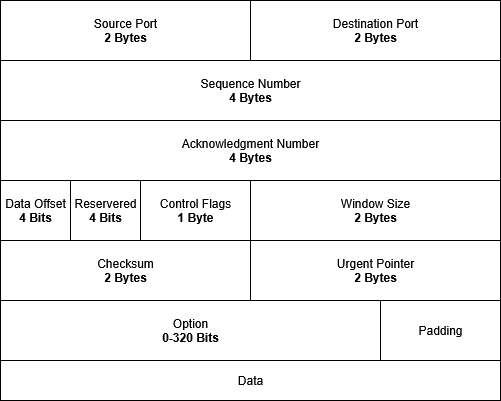
\includegraphics[alt={A block diagram of the TCP header format, detailing its fields and their sizes.}, height=8cm]{./images/tcp_header.png}
	\caption{The TCP header}
	\label{fig:tcp_header}
\end{figure}
The TCP header, Figure~\ref{fig:tcp_header}, encodes the functionality of TCP.
It follows the IP header in a datagram. The header is usually 20 bytes long but
can be extended using options. It begins with the source and destination port, which
together with the source and destination addresses, are used to identify the connection.
The next two fields in the header are the sequence and acknowledgement numbers. The
sequence number refers to the first data byte in the data segment.
If the SYN flag is set, this is the beginning of a new connection and the sequence
number in this case refers to the initial sequence number (ISN). The acknowledgement
refers to the next sequence number the receiver is
expecting to receive, at the same time acknowledging that all sequence numbers
up to this point were received. Next is the data offset field, indicating where
the data begins. The reserved field following this must be 0. After this is the
1-byte flags field
\begin{itemize}
	\item \textbf{URG} Urgent pointer field is set
	\item \textbf{ACK} Acknowledgement field is set
	\item \textbf{PSH} Push function, requesting that buffered data is sent immediately to the receiver
	\item \textbf{RST} Reset the connection
	\item \textbf{SYN} Synchronize sequence numbers
	\item \textbf{FIN} Sender is done sending data
\end{itemize}
The 2-byte window field specifies the number of bytes that may be in-flight at any one
time. This is the specified size of the sliding window that is used for flow
control purposes. Following the window field is a 2-byte checksum field, used for
detecting corruption of the TCP-header, data payload as well as a pseudo IP header,
containing information about the source and destination addresses, as well as the
protocol number and TCP packet length. In case the URG bit is set in the flags field,
the 2-byte urgent pointer header field indicates where the urgent data ends. Finally,
the options field contains extension to the normal TCP header, containing among other, options
for maximum segment size and multipath TCP~\cite{rfc8684}.

To ensure reliable delivery of TCP segments, each segment is assigned a sequence number.
This allows the receiver to reconstruct segments delivered out of order and additionally
detect missing segments. The receiver sends acknowledgments, containing the next expected
sequence number, to signal to the sender that the data was successfully received.
The sequence number is a 32-bit number, with the initial sequence number (ISN)
selected randomly at the time when the TCP connection is established. This ensures that
sequence numbers from stale connections have a low probability of overlapping with
any active connection~\cite{rfc793}.

The TCP connection is established via a three-way handshake. The client sends
a TCP packet with the SYN bit set in the flags field. This packet contains the
client's ISN. The server responds with a packet with the SYN and ACK bit set,
acknowledging the client's sequence number as well as providing the servers ISN.
Finally, the client responds with an ACK, acknowledging the servers ISN. Following
this the client and server are synchronized, and communication may begin. A peer
may terminate its side of the connection by sending a FIN packet, signaling to
the other endpoint that one side has closed its side of the communication. The
closed endpoint may continue receiving data until the other endpoint also closes
its side~\cite{rfc793}.
\subsubsection{User Datagram Protocol \label{UDP}}
\label{sec:udp}
\begin{figure}[b]
	\centering
	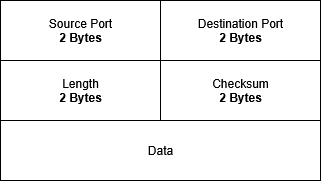
\includegraphics[alt={A block diagram of the UDP header format, detailing its fields and their sizes.}, height=4cm]{./images/udp_header.png}
	\caption{The UDP header}
	\label{fig:udp_header}
\end{figure}
UDP, which was defined by RFC 768, is designed to
enable programs to transmit self-contained messages, known as datagrams, over a
packet-switched network. UDP is designed to run on top of IP~\cite{rfc791},
using IP addresses and port numbers for addressing. UDP is by design connectionless,
providing no guarantees for datagram delivery, duplicate datagrams or in-order
delivery. In exchange, the UDP aims to minimize the overhead present in the protocol.
As UDP is connectionless there is no need to establish a connection via a handshake,
instead datagrams can be transmitted directly, and they should be designed in
such a way that they can stand on their own. The UDP header, as seen in Figure~\ref{fig:udp_header}
is only 8 bytes long,
consisting of the source and destination port, as well as the length of the datagram
and a checksum to verify the received datagram~\cite{rfc768}. Even though UDP has
a checksum field its use varies depending on the implementation. Some implementations
may discard the datagram or alternatively pass it along to the application with a 
warning, as UDP provides no way to recover from broken datagrams~\cite{compute_rnetworking}. The minimal UDP
header (8 bytes) combined with the lack of a handshake makes UDP a protocol with
the bare minimum needed for datagram transfer.
Generally, UDP is used for applications where low latency is a requirement, and some
amount of packet loss is deemed acceptable. It is then up to the application layer to
handle missing, reordered or duplicate datagrams.

\subsection{Streams}
\label{sec:streams}
A data stream is defined as a set of digital signals that is used to transmit
information~\cite{data_stream}. In practice, when talking about internet
transport protocols, a data stream refers to an ordered series of bytes that is
used to transmit information. For TCP this holds true, even though TCP splits
the transmitted data into packets, from the application point of view the
information is a stream of bytes. In comparison, UDP does not offer this same
abstraction, as each datagram exists independently of one another, but a series
of these datagrams could be seen as a type of data stream, albeit an unordered one.
Having only one stream per connection can lead to issues in the transport layer, such as HOL-blocking,
which is discussed in Section~\ref{sec:hol}. The solution of opening multiple
connections comes with the drawbacks of large overhead and resource consumption for
the peers, with each connection taking up a separate socket on the client machine.
As a result, protocols have emerged that aim to extend the data stream capabilities
of TCP and UDP, and in the process solve some of the issues present in these legacy
transport protocols.

\subsubsection{SST}

SST was introduced in ~\cite{sst} with the aim
of extending TCP semantics by introducing a hierarchical structure, allowing
child streams to be created on top of an existing stream. These streams can
be created without having to set up new connections, making them much more lightweight
than the TCP equivalent of opening multiple connections. SST supports multiplexed streams, allowing the streams
to exist in parallel, alleviating the issues of HOL blocking as each stream uses
independent flow control. SST also supports independent stream prioritization
as well as reliable and best effort (unreliable) delivery~\cite{sst}.

There were three primary reasons for creating the new protocol, SST, that splits
a single connection into multiple data streams. First, some protocols provide
multiplexing on top of TCP but suffer from HOL blocking as loss will block all
data transfers until retransmission. This issue arises as reliable communication
protocols guarantee that all bytes will be delivered in order, without any missing
chunks. Retransmissions, especially in high latency environments, causes delivery
delays for all of the data in the affected stream, or in the case of TCP, the
whole connection. Secondly, while
TCP is better suited for long connections and large data transfers, UDP excels
in short communications where the overhead of setting up connection via TCP's three-way
handshake provides significant overhead.  Finally, some protocols such as HTTP/1.0
have bad utilization of network resources, as they are designed to run on top of TCP
and open a new TCP connection for each resource that is loaded. This
was somewhat remedied in HTTP/1.1 with the serializing of requests over one connection,
but at the time of the SST's creation it had yet to be widely implemented~\cite{sst}.

As can be seen in Figure~\ref{fig:sst_arc}, the SST architecture consists of three
parts, the Stream, Channel and Negotiation Protocols. The Channel Protocol is responsible
for the delivery channel providing the best-effort delivery service, congestion control
and packet sequencing. The Negotiation protocol is responsible for setting up the channel
and negotiating protocol details. Most interesting is the Stream Protocol, building on
top of the other protocols to implement the Stream structure that SST is based upon.
SST implements the concept of child streams. Child streams are created on top of
a parent stream but are otherwise equivalent to the primary stream in all but name.
Child streams allow multiple streams to exist on top of one connection, and they
are designed to be lightweight. This mitigates the issue of HOL blocking between streams,
as loss on one stream still enables the other streams to keep transmitting while
the erroneous stream independently recovers. SST also implements a second type of stream,
while the normal stream is semantically like TCP, the second stream type, the ephemeral stream, is closer
to UDP. Ephemeral streams allow the application to have short communications as part
of a larger connection, without any additional overhead~\cite{sst}.


\begin{figure}[h]
	\centering
	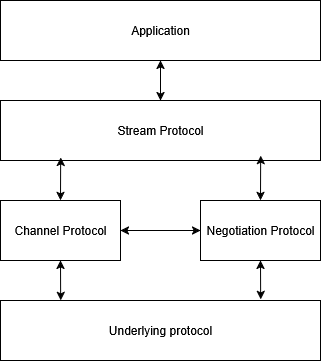
\includegraphics[alt={Diagram of the SST architecture.}, height=8cm]{./images/sst.png}
	\caption{The SST architecture}
	\label{fig:sst_arc}
\end{figure}

\subsubsection{SCTP}

The Stream Control Transmission Protocol (SCTP), was first defined in RFC 4960~\cite{rfc4960},
which was then later updated by RFC 9260~\cite{rfc4960}. SCTP was originally implemented
to carry Public Switched Telephone Network (PSTN) messages but was later standardized
into a general-purpose transport protocol. SCTP is a connection-based protocol, with connections
referred to as associations, and is designed to be run on top of IP. As a contrast
to TCP, which is designed to transport a byte stream, SCTP focuses on delivering individual
messages between applications. A message is sent on one end in one operation, and
the whole message is received on the other end, in one operation. A series of these
messages then form the stream inside SCTP. SCTP natively supports multiplexing of these streams, addressing TCP's issue
of HOL blocking. This is a significant improvement for PSTN messaging, where control
messages must not be delayed by data loss in other streams~\cite{rfc9260}.

In SCTP user messages are split into SCTP DATA chunks, which are bundled together
with SCTP Control chunks, together with a common header to form the SCTP packet. While
there may be multiple chunks inside one SCTP packet, each chunk only contains the data
of one message. Multiple sequences, streams, of these chunks may be sent in parallel
over one association, enabling multiplexed streams. SCTP supports both ordered and
unordered message streams, allowing messages to potentially be delivered out-of-order,
which may be preferable for certain kinds of data, such as control data~\cite{rfc9260}.

SCTP supports multihoming, allowing the protocol to simultaneously bind to multiple
different addresses and ports. This improves resilience, allowing the traffic to migrate
to a backup path in case the primary network path is experiencing issues. This migration
allows continued communication without breaking the association~\cite{rfc9260}.

\subsection{HTTP and its evolutions}

The Hypertext Transfer Protocol (HTTP), is a protocol stemming from the early days 
of the World Wide Web, defining a protocol that would allow a server and a client
to talk to each other. HTTP allows a client to request different resources from a 
web server, such as JavaScript, CSS, images, multimedia files or any number of different resources.
The high-level idea of HTTP is that a client requests a resource from the server,
and the server, if possible and permitted, responds with the requested resource.
HTTP defines the formats of these messages, which are written in American Standard Code for Information Interchange (ASCII),
making the message human readable directly on the wire, without having to interpret 
them. There are a set of HTTP request methods defined for the message, such as
the GET method for requesting a resource, and POST for sending data to the server~\cite{compute_rnetworking}.

A comparison of HTTP version can be seen in Table~\ref{tab:http_versions}. 
The first version of HTTP, HTTP/1.0 was defined in RFC 1945~\cite{rfc1945}. HTTP/1.0
used non-persistent connections and had no concept of multiplexing over a single connection.
It was a basic protocol, working on a request-response principle, with each request opening
its own TCP connection. HTTP/1.1 defines three request methods. GET to request data
from the server, POST to post data to the server and HEAD, which is similar to GET,
but requests that only the HTTP header be returned in the response, omitting the
body from the response~\cite{rfc1945}. What is notable for HTTP/1.0 is that it
did not suffer from the HOL-blocking of TCP, unlike most of its successors. Because each
request opened a new TCP connection, there was no concept of HOL blocking between requests as the
requests were entirely independent of one another. However, this was not very efficient
resource usage, as perform multiple three-way TCP handshakes to load a simple web page
added significant overhead.

\begin{table}[h]
	\centering
	\caption{Comparison of HTTP Versions}
	\label{tab:http_versions}
	\begin{tabular}{lllll}
	\textbf{Version} & \textbf{HTTP/1.1} & \textbf{SPDY} & \textbf{HTTP/2} & \textbf{HTTP/3} \\
	\textbf{Transport}    & TCP     & TCP & TCP & QUIC    \\
	\textbf{Multiplexing} & Pipelining    & Over TCP & Over TCP & QUIC multiplexing    \\
	\textbf{Compression}  & No    & SPDY specific & HPACK & QPACK    \\
	\textbf{Server Push} & No & Yes & Yes & Yes \\
	\end{tabular}
\end{table}

HTTP/1.0 was iterated upon and became HTTP/1.1, which was initially defined in
RFC 2616~\cite{rfc2616}. HTTP/1.1 improved upon HTTP/1.0, adding support for several
new features. First, persistent connections allow multiple requests to be sent over one connection,
cutting down on the number of connections that need to be opened to load a set of resources.
Second, pipelining allows multiple requests to be made at one time, without having to wait for the
response to the previous request. This was not quite yet true multiplexing, as the responses
need to be returned in the same order as the request were made, causing HOL blocking
of subsequent requests in case of loss~\cite{rfc2616}. Third, with the Introduction
of HTTP over TLS, HTTPS, it was now possible to set up more secure, encrypted communications,
instead of transmitting data in cleartext~\cite{rfc2818}.
\subsubsection{SPDY}

The SPDY protocol was designed by Google to improve latency of web pages, as compared
to HTTP/1.1. The SPDY protocol was designed to work as an extension to HTTP/1.1,
slotting into the session layer and largely defining how HTTP traffic is sent over the
wire, with some additional improvements to the HTTP protocol. In practice SPDY
introduced three improvements, multiplexed streams, header compression and server push capabilities~\cite{spdy}.

SPDY introduced multiplexing of HTTP streams, allowing for an unlimited number
of multiplexed streams over one TCP connection. The multiplexing works by splitting
the data into frames, which are interleaved and transmitted over a single TCP connection,
as can be seen in Figure~\ref{fig:http_mux}. As compared to HTTP/1.1's pipelining,
the true multiplexing of SPDY allows the server to respond to requests in any order,
instead of being forced to follow the specific request order. This allowed for a second improvement,
where a client could attach a priority value to the requests, signaling to the server
which resources should be prioritized, especially in congested channels. To limit
the number of bytes that must be sent over the wire SPDY implemented HTTP header
compression, sending the header in a compressed format instead of ASCII. Additionally,
SPDY added server push and server hint features. Server push allows the server to
send a resource to the client, without the client having request the resource first.
Server hint is similar to server push, but instead of sending the resource, the
server sends a hint to the client with a suggestion that the client should request
a specific resource~\cite{spdy}.

\begin{figure}[h]
	\centering
	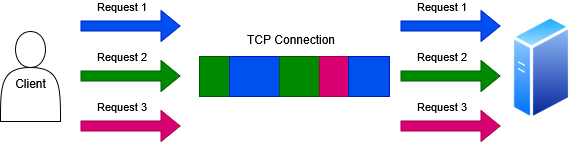
\includegraphics[alt={Block diagram of HTTP multiplexing.}, height=3cm]{./images/http_multiplex.png}
	\caption{HTTP multiplexing}
	\label{fig:http_mux}
\end{figure}

\subsubsection{HTTP/2}

HTTP/2 is standardized in RFC 9113~\cite{rfc9113}, is the evolution from HTTP/1.1.
It implements some of the ideas from SPDY, with the original specification for
HTTP/2, RFC 7540~\cite{rfc7540} containing acknowledging for the contributions made by the SPDY
team. The HTTP/2 protocol uses the same HTTP semantics as HTTP/1.1, but like SPDY
improves on the transport of the HTTP data between endpoints. HTTP/2 implements
streams and stream multiplexing, stream prioritization, header compression and
server push capabilities. Like SPDY, HTTP/2 supports multiple independently
multiplexed streams, allowing multiple parallel requests over one TCP connection.
Stream priority allows the client to signal which requests are more important to
be filled, and in case no priority is given, the server may choose to determine
priority based on other information~\cite{rfc9113}. For header compression, HTTP/2 implements a
dedicated compression algorithm called HPACK, defined in RFC 7541~\cite{rfc7541}.
HPACK not only implements compression, but the algorithm also helps in reducing
redundant header fields, by preventing the same static header fields from
being sent repeatedly ~\cite{rfc7541}. HTTP/2 supports server push capabilities,
allowing the server to send unprompted resources to a client, usually by estimating
the requests that the client likely will make in the future, in that way improving
latency~\cite{rfc9114}.

Even though HTTP/2 implements stream multiplexing, it still suffers from HOL blocking
since HTTP/2 streams are created on top of a single TCP
connection. This means that the requests won't block each other, but in case of
packet loss, the TCP HOL blocking will cause all requests to stall while waiting
for ~\cite{rfc9113}. This highlights the fact that despite improvements in the
HTTP protocol, the HOL blocking issue may not be solved as long as the protocol
is running on top of TCP.

\subsubsection{HTTP/3}

HTTP/3, as defined in RFC 9114~\cite{rfc9114}, is as of writing the latest evolution
of the HTTP protocol. It was specifically designed to be run on top of QUIC,
taking advantage of the improvements offered by the QUIC transport protocol. Like HTTP/2,
the HTTP semantics stay largely the same, but improvements are made to take advantage
of the new transport. HTTP/3 includes support for transport level multiplexing,
transport level encryption and connection migration. The most significant advantage
offered by HTTP/3 is the improvements to transport level HOL-blocking. Because HTTP/3
takes advantage of native QUIC streams for its multiplexing, which are entirely independent
on the transport level, packet loss won't affect unrelated streams. This allows
HTTP/3 to take full advantage of multiplexing requests to load resources, without
bottlenecking from the transport layer. QUIC offers an improved connection set up
time as compared to HTTP/2, as HTTP/2 uses TCP + TLS, requiring multiple RTTs to
establish a secure connection. HTTP/3 utilizes the fact that QUIC has the TLS
handshake integrated into the QUIC transport handshake, potentially reducing
connection set up time to 1 RTT. In some cases, it is even possible to use 0-RTT
data transfer to instantaneously transfer data without waiting for the connection
to be set up. Connection migration of QUIC allows connection to stay active for mobile
users, even in the face of network changes~\cite{rfc9114}. As with HTTP/2, HTTP/3 uses header compression,
but HPACK has been replace by QPACK, which improves on HPACK by better taking advantage
of QUIC's features, improving HOL blocking issues with only a slight degradation
in compression rate~\cite{rfc9204}.


\subsection{TLS}
\label{sec:tls}
The Transport Layer  Security (TLS) protocol is an evolution from the Secure Socket Layer (SSL)~\cite{rfc6101} protocol.
TLS aims to secure communication between two endpoints. The TLS protocol provides three
properties to data communication. First, authentication: the server side of the
communication is always authenticated, and the client side may optionally be
authenticated. Second, confidentiality: TLS ensures that data sent between the
endpoints is encrypted, ensuring that only the intended recipient can
decrypt and read the data. Finally, integrity: data transmitted through
a TLS tunnel cannot be tampered with, without alerting the recipient~\cite{rfc8446}.

The TLS protocol consists of two components, First, the handshake protocol is used to
establish the connection, being responsible for authentication, negotiation and creating
the key material used for encryption. Second, the record protocol is responsible
for encrypting and transmitting the data. The name comes from the fact that the data
to be transmitted is split into a series of records, all of which are individually
encrypted and transmitted. The TLS protocol is designed to be a general-purpose
security protocol, as it only requires to be ran on a reliable transport, and in
principle any application protocol may be run on top of TLS~\cite{rfc8446}.

The TLS handshake is the most important part when establishing a TLS session. In
TLS 1.2 and earlier the handshake required 2 RTTs before application data could be sent
securely, but since TLS 1.3 the handshake has been streamlined into 1-RTT, with the
possibility of 0-RTT data transfer, at the cost of perfect forward secrecy. The TLS 1.3
handshake is outlined in Figure~\ref{fig:tls_handshake} where the asterisk indicated optional
or alternative parts of the message, curly brackets indicate handshake secret protection and
square brackets indicate full application protection of data. The handshake begins with a ClientHello message,
containing a nonce, the protocol version and
either a pair of Diffie-Hellman key shares or a set of pre-shared key labels. The server responds
with a ServerHello, containing key shares, certificate if it is used in authentication of the server
and possible extensions, such as a CertificateVerify request in case the server requests that the client
be authenticated via a certificate as well. The certificate and CertificateRequest as
well as Extensions are protected with keys derived during the handshake process. These
are different from the secrets used to protect application data and do not guarantee
perfect forward secrecy. The combination of ClientHello and ServerHello is used to
create the shared keys. Finally, the client responds, acknowledging that the process is finished~\cite{rfc8446}.

\begin{figure}[h]
	\centering
	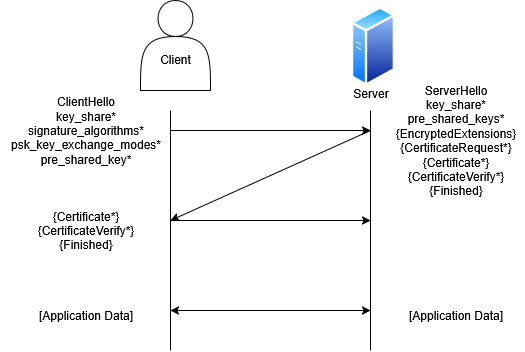
\includegraphics[alt={Diagram of TLS handshake between a client and a server}, height=9cm]{./images/tls_handshake.png}
	\caption{The TLS 1.3 Handshake}
	\label{fig:tls_handshake}
\end{figure}

Normally the handshake adds additional overhead to connection set up. With TLS 1.2 and
lower adding an additional 2+ RTTs of latency, and TLS 1.3 adding 1-RTT of latency.
However, the QUIC protocol integrates the TLS 1.3 handshake into the transport layer protocol,
allowing both handshakes to be made in parallel, negating the latency impact, but more
on this in Chapter~\ref{sec:quic}. Once the handshake is finished and the TLS session set up,
the record protocol takes over. The record layer splits the application data into
appropriate chunks, which are then encrypted and integrity protected. Finally, the record layer transmits
these records via the underlying, reliable transport.

The first versions of TLS, TLS 1.0 and 1.1, defined in RFC 2246~\cite{rfc2246} and
RFC 4346~\cite{rfc4346}, improved upon SSL but were deprecated in 2021 via RFC 8996~\cite{rfc8996},
due to the fact that these algorithms rely on weak cryptographic algorithms. The TLS 1.2
protocol improved upon its predecessor by introducing more secure cryptographic algorithms and
authenticated encryption~\cite{rfc5246}, and removing backwards compatibility with
SSL via RFC 6176~\cite{rfc6176}. Finally, as mentioned earlier in this section,
TLS 1.3 is the latest version of the TLS protocol. It removed support for legacy
cryptographic algorithms, added the 1-RTT handshake and 0-RTT data transfer, among other
cryptographic improvements~\cite{rfc8446}.

\subsubsection{DTLS}

As mentioned in Section~\ref{sec:tls}, the TLS protocol is designed to run on top
of a reliable transport protocol. However, it is quite common for applications to run on top
of UDP, which as mentioned in Section~\ref{sec:udp}, makes no guarantees for reliability.
To solve this problem and provide protection for datagram-based applications,
Datagram Transport Layer Security (DTLS) is designed to overcome the challenges
of securing an unreliable transport. There are four main reasons the TLS cannot
be used directly on top of UDP. First, TLS uses an implicit sequence number as a
nonce, meaning that TLS records being delivered out of order causes the decryption
process to fail. Second, the TLS handshake is rigid, the right messages must arrive
in the right order for the handshake to succeed. Third, handshake messages may be 
larger than one datagram, causing fragmentation. Finally, UDP is susceptible to
Denial-of-Service (DoS)~\cite{rfc9147}.

To handle packet loss, DTLS uses a retransmission timer to enable retransmission of
lost packets, such as part of the handshake. Reordering is mitigated by assigning
an explicit packet number, enabling the receiving party to process the received
messages in the correct order. DTLS adds support for fragmentation of handshake messages,
the sending party can split the handshake message into multiple parts that all fit
inside single datagrams, and the receiving party can then reassemble the handshake message
from the fragments. To combat DoS attacks,  DTLS implements a HelloRetryRequest message,
which contains a cookie, that then must be included in the ClientHello message
to be accepted by the server. Optionally, DTLS includes replay detection and protection~\cite{rfc9147}.

DTLS is designed to be as close to TLS as possible in capabilities and functionalities.
DTLS follows TLS versioning, with the latest, DTLS 1.3, being defined in RFC 9147~\cite{rfc9147}.
Like TLS 1.3, DTLS 1.3 implements the improved 1-RTT handshake, enforces stronger
cryptographic algorithms than earlier versions and adds support for 0-RTT data transfer,
however 0-RTT data transfer requires that replay protection is enabled on the connection~\cite{rfc9147}.

\subsection{DFS}

Distributed File Systems (DFS) allow clients to communicate with servers, enabling
the clients to manipulate the files as if they were stored on their local machine.
DFS's abstract away the complexities of distributed data access, exposing a set
of file operations to the clients, allowing them to create, delete, read and write files among other operations.
The DFS ensures consistency, reliability and access between different
clients and access points~\cite{os_concepts}. Currently, the two most widely adopted
distributed file systems are the Server Message Block (SMB)~\cite{smb2} and the
Network File System (NFS)~\cite{rfc7530}. Both protocols provide file system access
over a network, but they differ in design, environment and features.

\subsubsection{Server Message Block}

The Server Message Block (SMB) protocol is a stateful protocol, and is a protocol designed for
sharing files, printers and other resources over a network. It was originally created
in the early 1980s and later adopted and extended by Microsoft~\cite{samba_myths}.
The protocol has undergone several iterations since that time. While the underlying
concepts of SMB have stayed the same, later revisions, that is SMB version 2.0 and forwards,
differ heavily from earlier versions. SMB 2.0 introduced different packet formats, and reduced
the chattiness of the protocol, among other improvements. SMB 3.0 introduced encrypted traffic,
multichannel support and integration with RDMA in the form of SMB Direct. Since SMB 3.1.1 the
protocol has added support for using the QUIC protocol as an alternative transport~\cite{smb2}.

The main distinguishing characteristics of the SMB protocol is its stateful design.
The server maintains information about the state of a session, such as file handles,
locks and leases, over the lifetime of a session. This allows the SMB protocol to
guarantee consistency and helps in coordinating multiple, concurrent clients. As 
the development of the SMB protocol has largely been a result of Microsoft's effort,
the protocol is deeply integrated into the Windows ecosystem,
supporting NTLM and Kerberos authentication, and integrates as part of Active Directory Domain
services~\cite{smb2}.

\subsubsection{Network File System}

The NFS protocol was introduced by Sun Microsystems in 1984, aiming to be a protocol
for enabling remote access to filesystems between different UNIX machines. NFS was
designed to be a simple and open filesystem, making it easy to port to different
machines. In contrast to the SMB protocol, the NFS protocol was designed to be a 
stateless protocol. This simplifies processing, as each request contains all necessary
information to complete the request, and if the request fails the client may
simply try again. Recovery from error states is simpler as no sessions have to be
re-established. The stateless  design come with drawbacks,
for example two concurrent clients trying to write the same file could cause the
writes to be interleaved, causing unintended outcomes, as the writes are simply
processed in the order they arrived~\cite{nfs_design}.

Over time the NFS protocol has evolved, with the latest version NFSv4.2 being
defined in RFC 7862~\cite{rfc7862}. NFSv4 introduced stateful capabilities into the protocol, and
includes features such as file locking, multipath and compound operations, alongside performance
improvements and improved authentication support for stronger security~\cite{rfc7530}.
NFSv4.1 introduced NFS sessions and parallel access to data, as well as improving support
for clustered solutions~\cite{rfc8881}, while
NFSv4.2 introduces support for server-side operations, and sparse files~\cite{rfc7862}.

\begin{table}[h]
	\centering
	\caption{Comparison of SMB and NFS}
	\label{tab:smb_nfs}
	\begin{tabular}{lll}
	\textbf{Protocol} & \textbf{SMB} & \textbf{NFS} \\
	\textbf{Environment}    & Windows     & UNIX    \\
	\textbf{Resources} &  Files, directories, printers, network resources   & Files and directories     \\
	\textbf{Sessions}  & Stateful  & Stateless v2/v3, Stateful v4    \\
	\end{tabular}
\end{table}

Table~\ref{tab:smb_nfs} gives an overview of the major differences between SMB and
NFS. SMB provides many different features, a natively stateful protocol for sharing
all kinds of resources, and a solution that is very Windows centric, with UNIX based
system requiring a third-party solution for support, such as Fusion SMB or
Samba. In comparison, NFS is a lightweight, easy to set up protocol that is purely
focused on file and directory sharing, and which is integrated into many
different UNIX based operating systems.
\clearpage

\section{QUIC}
\label{sec:quic}
The Internet's underlying infrastructure is in a state of constant evolution,
driven by a demand for decreased latency, increased throughput requirements and
a need for improved security. For many years now, TCP has been the de-facto
solution for reliable and secure (when combined with TLS) communications. However,
TCP was developed in a time when security and latency were not primary considerations,
at least not in the same way as in today's landscape. Over the years there have
been efforts to enhance TCP, such as multipath TCP~\cite{rfc8684} and using both
TCP and TLS in HTTPS~\cite{rfc2818} to improve security. This section of the thesis
will cover QUIC, a transport protocol developed to overcome the limitations of TCP
and improve performance~\cite{quic_transport_protocol_design}.

The importance of the QUIC protocol is not to be underestimated. It represents
a substantial change to the internet's transport layer, the first one in over
two decades. QUIC was initially developed by Google, and then later standardized
in RFC 9000~\cite{rfc9000}. QUIC is designed to address the issues experienced
by TCP, with a focus on optimizing for web traffic, with the development being
largely done hand-in-hand with HTTP/3. The main issue of TCP that needs to be overcome is the
HOL blocking, but  QUIC also aims to improve on other aspects of the protocol,
such as integrating the TLS handshake into the transport handshake. A decision
that was made for QUIC specifically was to move the protocol out of the kernel
space and into the user space, allowing for rapid development and innovation~\cite{quic_transport_protocol_design}.

This chapter of the thesis will outline the limitations of TCP that led to the
development of QUIC and give an overview of the architecture and functionality of
the protocol.

\subsection{The motivation for a new transport protocol \label{quic_motivation}}
TCP is a cornerstone of modern internet infrastructure. It has been the go-to
protocol for reliable communications for more than 40 years, ensuring connectivity between users and hosts
since its inception. However, as the design of TCP is largely influenced by the
landscape of when it was created, many of the improvements that have been made to TCP,
such as security, have had to be built on top of TCP, as these were not considerations
at the time of TCP's inception. Today's internet landscape, with real-time content,
hyper-mobile users and increased demands on not only latency, but also privacy and security, have exposed
some of the limitations imposed by the TCP stack. This section will outline the
key issues that prompted the development of a new, modern protocol: QUIC.

\subsubsection{Head-of-Line Blocking}
\label{sec:hol}
As discussed in Section~\ref{sec:streams}, TCP is negatively affected by HOL blocking.
To get around this limitation, modern
network protocols, such as HTTP/2~\cite{rfc9113}, have introduced measures to
combat this issue. HTTP/2 introduced multiplexing of multiple requests over one
connection, allowing multiple application-level streams, for example for different
resources such as images or JavaScript, to be multiplexed over a single TCP
connection. This means that HTTP/2 managed to mitigate application-level HOL
blocking, which was an issue in earlier versions of HTTP. However, HTTP/2 still
suffers from transport level HOL blocking, as the multiplexed stream is
sent over a single TCP connection. As a result, a single lost packet in the TCP
stream still causes all other unrelated streams over the same connection to stall,
even if their packets were successfully delivered, until the offending packet
is retransmitted and received. This in practice means that many of the improvements made
by HTTP/2 in this regard are negated by the issues of TCP, particularly in lossy or high latency
environments~\cite{http2_vs_1}.

\subsubsection{Handshake Delay}
A limitation of the TCP stack is the delay caused by the TCP handshake. As discussed
in earlier chapters, establishing a TCP connection is done via a three-way handshake
(SYN, SYN-ACK, ACK). This handshake incurs one Round-Trip Time (RTT) of delay. In
addition, most applications use TLS for security, and historically the TLS 1.2 handshake
and set up add two additional RTTs of delay. While network bandwidth is ever increasing,
much of the communication done on the internet consists of short dialogues, that
are significantly impacted by the additional latency brought on by the TCP plus TLS
handshake~\cite{quic_transport_protocol_design}.

Some of the latency brought on by the TLS handshake is addressed by TLS 1.3, adding
support for 1-RTT and 0-RTT handshakes, at the cost of perfect forward secrecy~\cite{rfc8446}. Even with
these enhancements, the TCP plus TLS handshake takes a minimum of 1.5 RTTs before data can be
transmitted, due to the separation of the connection and security handshake. There is
an extension to TCP called TCP Fast Open (TFO) that enables data to be sent during
the TCP handshake, in the SYN and SYN-ACK packets. For TLS this means that
the ClientHello can be carried in the initial SYN packet~\cite{rfc7413}. The main problem
with TFO is that a significant amount of middleboxes will drop TCP packets with
unknown SYN data or options. If any of these devices are on the path between the
endpoints, using TFO is simply not possible~\cite{fast_open_problem}.

\subsubsection{Protocol Ossification}
A big hurdle in deploying new protocols and extensions to existing ones
is the protocol ossification of protocols on the internet. There exists a large number of different
middleboxes, such as Network Address Translators (NATs) and firewalls that are all
part of the network. These devices may be overly conservative, dropping or 
modifying packets that do not conform to their assumptions. This is already an
issue for TCP enhancements, and entirely new protocols have no chance of reaching
their destination, without explicitly adding support in all the middleboxes on the path.
To get around this, protocol designers must design their protocols from the ground
up to be resistant against middlebox interference, such as is the case with QUIC encapsulating
its protocol inside UDP as an anti-ossification measure~\cite{Ossification}.

A related issue of rolling out enhancements to existing protocols is that the
network stack tends to be part of the OS kernel. The networking
stack is tightly coupled with the OS, requiring OS updates or upgrades to implement
changes to existing protocols. With today's upgrade frequency, it can take years
to roll out simple changes to the networking stack. QUIC moves the implementation of the 
protocol into the user space, improving the speed of development and deployment,
and opening up the space for multiple actors to create their own implementations of
the protocol~\cite{quic_transport_protocol_design}.

Additionally, the TCP header is limited to 60 bytes, of which 20 bytes is taken
up by the mandatory fields of the header, which leaves 40 bytes of space for the options.
However, all existing options consume space, and seeing as the space is so limited,
it is not difficult to exceed the available space. For example, SACK can use as much
space as is available, or timestamps that take up 10  bytes, so one quarter of
the total available space. In practice this leaves very little space for extending
the protocol, further increasing the difficulty of implementing new features~\cite{ietf-tcpm-tcp-edo-15}.

\subsection{Background and evolution}
As discussed in Section \ref{quic_motivation}, the combinations of TCP, TLS and HTTP/2 are
plagued by issues that are difficult to circumvent without major overhauls or extensions to
the individual protocols. Due to protocol ossification, this is increasingly difficult. With
this in mind, a new protocol was created, aiming to solve the issues of
HOL blocking, improve latency and circumvent protocol ossification. The result
was the protocol that would later be standardized into QUIC, early on known as gQUIC.
QUIC began development back in 2012, by Jim Roskind, an engineer at google. Initially
the motivation for developing a new transport protocol was to improve support for
the now deprecated SPDY protocol, which had initially been designed to run on top
of TCP~\cite{googleQUICDesign}. QUIC was designed to run over
UDP, by encapsulating the protocol frames into UDP datagrams, and encrypting the contents.
This way the protocol could effectively sidestep the issues of middlebox interference, allowing
for rapid deployment without any necessary modifications to existing infrastructure.
To combat the issue of HOL blocking, QUIC implements transport level multiplexing of
data streams, allowing multiple independent streams to exist over one connection.
Packet loss in any of the data streams would not affect any of the others, blocking
only one stream, while waiting for retransmission. QUIC uses a combined connection and
cryptographic handshake, minimizing the latency of establishing a new connection.
While TCP uses IP-port tuples to identify connections, this does not allow for changes in the
underlying network, such as might be the case for mobile users. If the IP or port
of the user changes during the lifetime of the connection,
the connection is dropped and must be reestablished. To combat this QUIC uses
Connection IDs to identify the connection, allowing the connection to resume when
there is some change in network. QUIC was widely deployed on Google's front-end servers,
and by 2017 it was already estimated that QUIC represented 7\% of global internet
traffic~\cite{quic_transport_protocol_design}. Since then, the adoption of QUIC has
been rapid and according to statistics by Cloudflare, QUIC makes up more than 30\% of web traffic~\cite{cloudflare_radar}.

QUIC was submitted to the IETF for consideration in 2016, and a working group
was created for the purposes of standardizing QUIC. The goal of the working group
was to create a general-purpose transport protocol that contained the benefits
of gQUIC. The custom cryptographic handshake was replaced with TLS 1.3, the packet header
was reworked into two types, a long and a short header. The header is mostly encrypted
to prevent middlebox interference. Loss detection and congestion control mechanics
were updated, flow control semantics were separated into per stream and per connection
limits and version negotiation was introduced to improve forward compatibility of the
protocol~\cite{rfc9000}. In the end the protocol was standardized in several RFCs.
RFC 9000~\cite{rfc9000} defines QUICs core transport mechanics, RFC 9001~\cite{rfc9001} defines the use of TLS 1.3
and RFC 9002~\cite{rfc9002} describes the loss detection and congestion control algorithms used by the
protocol. In addition, RFC 8999~\cite{rfc8999} defines some version-independent
properties of QUIC, aligning QUICK packets, headers and versioning between
different versions of the protocol. Following the standardization the adoption
of QUIC has been quick. Chromium, and by extensions all chromium-based browsers
has supported QUIC since before it was standardized~\cite{chromium_quic}. Both
Firefox~\cite{firefox_quic} and Safari~\cite{safari_quic} added support for QUIC
soon after the standards were published. QUIC has shown the viability and potential
of deploying network protocols to the user space, enabling rapid adoption without slow
OS kernel updates.

\subsection{Architectural Overview}

The QUIC protocol is designed to be a general-purpose, secure and multiplexed
transport protocol, working on top of UDP. In comparison to TCP, which usually
is part of the OS kernel, QUIC is typically implemented in the user space, enabling
quick iteration and deployment of protocol enhancements. This section describes
QUIC's position in the networking stack, the different architectural parts of the protocol
and the basic elements of the protocol's operations.

QUIC packets are directly encapsulated inside UDP datagrams. This design has both 
practical and implementational advantages. When deploying QUIC, the fact that the
wire image of QUIC packets is identical to that of UDP datagrams, means that they
pass seamlessly through middleboxes and firewalls, without suffering the adverse
effects of protocol ossification as is often the case in TCP. As discussed in Section \ref{UDP},
UDP is a barebones protocol, with the minimum overhead needed to transmit datagrams. This
works to the advantage of the designer when building a protocol on top of UDP, as
this give the freedom needed to implement entirely custom semantics, without risking
interference from the underlying protocol. UDP provides the basic datagram services
that are then enhanced by the QUIC protocol, ensuring a secure, reliable and performant
protocol~\cite{quic_transport_protocol_design}.

From an architectural perspective, QUIC incorporates three main layers, a transport
layer, a security layer and an application interface. From the bottom up, UDP provides
minimal mechanism for transmitting datagrams, without any guarantees. On top of this
QUIC implements its own transport layer, handling the multiplexing of data streams,
ensuring reliable and in-order delivery of data as well as connection management
mechanics~\cite{rfc9000}. QUIC's security layer is fully integrated into the protocol, using TLS 1.3
for encryption of on-wire traffic, as well as authentication and authorization of peers, ensuring
secure communication between endpoints. The security layer also protects most of
the packet header, leaving only the necessary info for routing and version control
visible on the wire~\cite{rfc9001}. The final layer exposes a standardized application
interface that can support virtually any application-layer protocol, the most prominent
one being HTTP/3~\cite{rfc9113}.

One of the main innovations made by the QUIC protocol is the concept of transport-level,
multiplexed and independent data streams. Any QUIC connection may contain one or multiple
data streams, handled entirely as their own independent object. This helps mitigate the
HOL blocking issues, as if the application is using multiple streams, when loss occurs on a stream,
only the stream on which the loss occurred will be blocked. While the lossy stream is
stalling and waiting for retransmission, the other streams can continue sending as 
normal. QUIC uses per connection limits for the number of streams and per stream
flow control limits~\cite{rfc9000}.

Connection management and identification in QUIC differs from the IP-port tuple
combination that is traditionally used in TCP for identifying connections. QUIC connections are identified via a
connection ID, which is independently selected by the endpoints. The purpose of the
connection ID is to allow the connection to survive changes in the underlying network, for example
when a mobile user moves from a local network to cellular. The migration is done transparently
and securely, allowing the application to continue operations without interruption or having
to reestablish the connection~\cite{rfc9000}.

\subsection{Packet and Frame Structure}

QUIC packets are contained inside UDP datagrams, and together with the encryption
and integrity protection provided this gives robust protection against protocol
ossification. As compared to TCP, where segmentation and reassembly of packets are
transparently done as part of the transport protocol and not accessible to the
application, QUIC defines a large set of different frame types for different,
distinct roles in connection establishment, data transfer and protocol logic
management. Depending on the packet type QUIC uses either a long header or short
header.

QUIC packets are divided into two general categories, those that use the long header
and those that use the short header. The long header is used during the establishment
of the connection, being used in the Version Negotiation, Initial, 0-RTT, Handshake
and Retry packets. The long header, as seen in Figure~\ref{fig:quic_header}, contains the
necessary data for these functions. The first bit of the long header is set to 1 to indicate
that this is a long header. The fixed bit following this is always set to 1, except
for Version Negotiation packets. The Long Packet type indicates the type of packet,
and the 4 type specific bits are dependent on the packet type. Following this,
the version ID field indicates the specific QUIC version this packet is using, and
finally the destination and source ID length and IDs contain the identifiers for
the source and destination of this packet. Following the header is, if relevant,
the specific packet type payload. In addition, the Initial, 0-RTT and Handshake
packet types include a packet number length and packet number field. In comparison,
the short header is more compact, reducing per-packet overhead. The Header Form bit
(set to 0 in the short header case) and the Fixed bit is the same as for the long
header. The Spin Bit that follows may be used to make on path estimations of
the RTT. Following the two reserved bits is the key phase bit, used to keep
track of the keys that are used to protect the packet. The packet number length
is the length of the packet number field minus one. Lastly is the destination ID
again indicating the recipient, the packet number used for protocols semantics
and finally the packet payload~\cite{rfc9000}.

\begin{figure}[h]
	\centering
	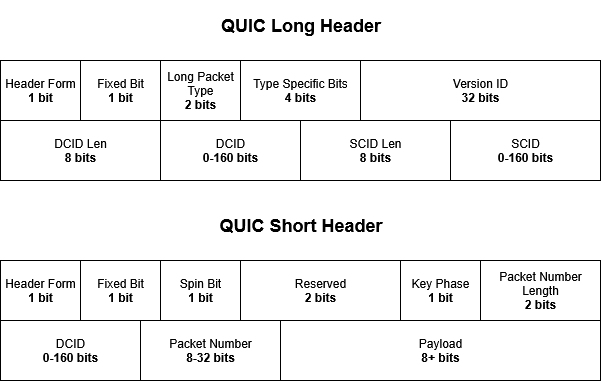
\includegraphics[alt={A block diagram of the QUIC short and long header format, detailing its fields and their sizes.}, height=8cm]{./images/quic_header.png}
	\caption{The QUIC header formats}
	\label{fig:quic_header}
\end{figure}

The long header packet type numbers differ between QUIC version 1 and version 2, as
is outlined in Table~\ref{tab:quic_long_header_types}. Initial packets are used to initiate the connection and transmit
the initial TLS handshake. The Handshake packet carries the subsequent
cryptographic messages, after the initial exchange. In case the connection attempt is
a resumption, the client may use the 0-RTT packet type to transmit encrypted application
data as part of the handshake, basing the encryption on previously established keys. The
Retry packet type may be used by the server to force the client to
validate its address~\cite{rfc9000}.

\begin{table}[h]
	\centering
	\caption{Table of QUIC long header types}
	\label{tab:quic_long_header_types}
	\begin{tabular}{lll}
	\textbf{Packet Type}		  & \textbf{QUIC v1} & \textbf{QUIC v2} \\
	Initial   & 0x00    & 0b01    \\
	0-RTT     & 0x01    & 0b10    \\
	Handshake & 0x02    & 0b11    \\
	Retry     & 0x03    & 0b00   
	\end{tabular}
\end{table}

In QUIC there is only one short-header packet type, known as the 1-RTT packet. It is
used for the bulk of communication, taking advantage of the more compact short
header to reduce overhead on the connection, which is useful for high-throughput
applications. The header is in part protected by header protection, preventing
interference by middleboxes on the wire.

QUIC uses the concept of frames to enable protocol functionality. The payload of
QUIC packets consists of one or more frames, and the frames can be of different types,
enabling the transmission of application data and control data in the same packet. Frames
allow the QUIC protocol to signal transport events between the peers. Arguably the most
important frame type is the data transmission frame, known as the STREAM frame. The stream frame
carries stream data associated with a specific stream. The STREAM frame contains
a stream identifier, byte offset and flags to track the state of the stream. The STREAM
frame implicitly creates a new stream in case the identifier is previously unknown.
The ACK frame is then used to acknowledge received packets. The ACK frame contains
one or more ranges of packet numbers that have been received, with possible gap values
indicating missing packets. This higher granularity enables the sender to only retransmit
the missing packets, lowering retransmission overhead in reordering scenarios. Other
important frame types include MAX\_DATA and MAX\_STREAM\_DATA for flow control
on the connection and stream level, PING frames to probe the peer and ensure that
the connection stays alive, CRYPTO frames for carrying TLS handshake data and CONNECTION\_CLOSE frames
to terminate the connection. These are the most important frame types, with an
extensive list being available in RFC 9000 chapter 19 Frame Types and Formats. Together,
these frames allow for great control of transport functionality, allowing for explicit
connection management~\cite{rfc9000}.

\subsection{Streams}

The QUIC protocol is designed around the concept of streams. Streams are an abstraction
of a byte-streams, that are used to transmit data between applications. Streams may
be either bidirectional or unidirectional, that is, from the perspective of one peer,
the streams may be read-only, write-only or read and write. Any single connection may contain one or
more streams, with the streams being multiplexed and entirely independent from one
another. Streams are designed to be lightweight, with minimal overhead. A stream can
open, close and transmit data in a single frame, or alternatively the streams
can persist for longer lengths of time, up to the lifetime of the connection. The number
of streams and the amount of data that may be sent over a single stream is constrained
by the flow control. The different streams are identified via a unique identifier inside a connection,
the stream ID, which is a 62-bit integer. The reasoning for using a 62-bit integer is
that the two remaining bits are used to distinguish between unidirectional and bidirectional
streams, as well as identify the initiator of the stream, which may be either the
client or server~\cite{rfc9000}.

The lifetime of a stream is explicitly managed by the peers. The stream is first
created by sending a stream frame, containing the stream ID of the stream that is
requested to be opened. Data transfer is done via STREAM frames, that carry the
application data that is to be transmitted. Once data transfer is complete, and
the application is done with the stream, it may be closed by sending a stream
frame with the FIN bit set or alternatively by sending a RESET\_STREAM to abruptly end the
stream, signaling that no further data will be sent. At the receiving end the receiver
can read data from the stream and may end the stream by sending a STOP\_SENDING frame,
signaling that no more data will be accepted on the stream~\cite{rfc9000}.

The design of QUIC streams is such that it directly addresses TCP's HOL blocking
issue. In TCP, the in-order delivery guarantee is implemented on an entire connection,
resulting in the whole connection stalling in case of a lost packet until the packet is
retransmitted and received. In comparison, QUIC building its streams on top of
UDP, has implemented an in-order guarantee per stream. That is, any lost packet
only blocks the specific stream that packet belonged to, allowing the other streams
that may exist on the same connection to keep transmitting while the erroneous
stream retransmits. This feature also works in the favor for control data,
as control frames are transmitted separately from the stream frames, they are not
affected by loss on any of the data streams~\cite{rfc9000}. An example of this advantage
in action is in the HTTP/3 protocol. Here each client request is mapped to its own
bidirectional QUIC stream, and unidirectional streams are used for control and
push streams. HTTP/3 implementations should support at least 100 concurrent streams
taking advantage of the multiplexing introduced by QUIC~\cite{rfc9114}. When a client
visits a web page, it may open tens of streams simultaneously, to fetch HTML, CSS,
JavaScript, images and fonts. If, for example, a packet containing part of an image is lost, QUIC
enables the HTML and CSS streams to continue delivering while the image stream recovers,
improving web page render times in lossy environments.

The lightweight  design of QUIC streams makes them suitable for short request-response
communications in other domains as well. DNS over QUIC takes advantage of the
stream semantics by creating a new QUIC stream for each request. Besides preventing
HOL blocking, DNS over QUIC takes advantage of QUIC's stream semantics by allowing
each DNS query to use a separate stream for communication. This allows the protocol
to cheaply process each request-response, forgoing the overhead of setting up a connection,
with its full handshake, instead creating a lightweight stream for the specific
communication, while still guaranteeing the reliable delivery of requests and responses.
The multiplexed streams also allow the server to process and respond to the queries
out-of-order, allowing multiple, simultaneous, outstanding queries at any one time~\cite{rfc9250}.

\subsection{Flow and Congestion Control}

To prevent fast senders or malicious actors from overwhelming the receive buffer,
the QUIC protocol implements flow control on two levels, a per-stream flow limitation
and a per-connection limitation. The receiver controls the amount of data that can
be sent on any one QUIC stream at a time, as well as over the connection as a whole.
The receiver also limits the number of concurrent streams that the sender may open,
preventing the overwhelming of the receiver with a large number of unique streams.
The limits are set during the handshake process, but they may be updated by sending
MAX\_STREAM\_DATA and MAX\_DATA frames to signal that the flow control limits have
been increased. A receiver may not reduce the flow control limits during the connection.
If the sender is faster than the receiver it may reach a state where it is unable
to transmit data due to either one of the limits. In this case the sender should
send a STREAM\_DATA\_BLOCK or DATA\_BLOCK frame to signal to the receiver that
there is outstanding application data waiting to be sent, but it is currently unable to send
due to the flow control limits. Similarly, the limit on the number of streams that
may be opened is set during the connection initialization phase. The limit may be
increased by sending a MAX\_STREAMS frame, and similarly to the data flow control limits,
the streams limits may only be increased, not decreased. The sender can signal to the
receiver that it would like to open more streams by sending a STREAMS\_BLOCKED frame~\cite{rfc9000}.
This granular control allows the protocol implementations to adapt the flow control
according to the environment, enabling improved performance especially in dynamic environments.

The QUIC protocol uses three different packet number spaces, separate for initial,
handshake and application data spaces. This is due to the
corresponding packets using different levels of encryption, ensuring that acknowledgements
sent in one packet number space does not cause retransmissions of packets of a different
encryption level. The packet numbers of QUIC are monotonically increasing, signaling
the order in which the packets were sent. That is, when retransmission occurs the
retransmitted packet uses the next available packet number instead of the same packet number.
To reconstruct reordered packets QUIC instead
uses a stream offset field inside the stream frames, to keep track of the correct
order of data. Loss detection in the QUIC protocol is then based on these packet
numbers. Loss can either be detected via acknowledgement-based detection,
if a packet that is considered in-flight and is unacknowledged, but a packet
sent after the potentially lost packet has been acknowledged, and enough time has passed
since the first packet was sent. Alternatively, a Probe Timeout (PTO) causes one or two
datagrams to be sent out, expecting a response to test the reachability of the peer~\cite{rfc9002}.

The QUIC protocol provides a set of generic signals that are designed to support
multiple different sender-side congestion control algorithms. A congestion algorithm similar
to TCP NewReno~\cite{rfc6582} is outlined in RFC 9002. However, a sender is free to
choose any one algorithm they feel suits their use case, such as CUBIC, given that they conform
to the congestion control algorithms outlined in RFC 8085~\cite{rfc8085}. One option
is to use QUIC packets which contain only ACK frames, as these do not count towards
the flow control limits, but the loss of these packets can be detected by the QUIC
algorithm~\cite{rfc9002}.

The algorithm outlined in RFC 9002 begins in slow start, setting the initial congestion
window to 10 times the maximum datagram size. When in slow start the sender increases
the congestion number by the number of acknowledged bytes, until packet loss is detected. This
means that the congestion window can double every RTT as long as all inflight packets
are acknowledged. When packet loss is detected, the sender enters recovery period.
During the recovery period the congestion window is reduced to half its current
size, and this reduction may be made instantly when entering the recovery period
or gradually using some other mechanism. Any additional loss detected during this
period does not affect the congestion window size. The recovery period ends once
the congestion window has been reduced to the new size, and the sender has sent
a packet and that packet has been acknowledged. From here the sender enters congestion 
avoidance. During the congestion avoidance period, the sender may at maximum increase
the congestion window by one maximum datagram size for each complete congestion
window that has been acknowledged. In case loss is detected the sender goes back
into recovery mode. In case persistent congestion is detected, that is the continuous
loss of all sent packets, the sender reenters slow start mode, and the process
starts over~\cite{rfc9002}.

In the QUIC algorithm there may be a situation where reordering of packets causes
the receiver to receive packets to which it does not have the necessary keys to
decrypt, such as handshake or 0-RTT packets arriving before the initial packets.
Loss of these packets may be ignored, unless an earlier packet from the same packet space
has been acknowledged, in which case the loss must not be ignored. When a probe
packet is sent it should not be blocked by the congestion controller, even if they might exceed the current
congestion limits, and these packets should also be accounted for as being in-flight. The
sender should pace the sending of its packets, as large bursts of packets may induce 
congestion or packet loss. A lack of application data or pacing on the part of the
sender may cause the congestion window to be underutilized. In this case the congestion
window should not be increased~\cite{rfc9002}.

\subsection{Connections}

The QUIC protocol is a stateful, connection-oriented protocol where the QUIC
connection functions as the shared state between peers. Connections are created
via a handshake, during which both the transport and security handshake is performed,
with the security handshake being based in TLS 1.3~\cite{rfc9001}. The handshake establishes
the connection, and the parameters for the connection are declared. The parameters
are individually decided by the peers, and the opposite peer needs to comply with
the conditions set. It is possible via 0-RTT data transfer to transfer application
data as part of the initial message, before the server has responded, and the server
may already start sending data before the final handshake message from the client.
This allows the protocol to exchange some security guarantees for improved latency
when establishing a connection~\cite{rfc9000}.

\subsubsection{Connections and Identifiers}
\label{sec:connections_ids}

From a connection standpoint one of the innovations made by the QUIC protocol, as
compared to TCP, which uses port-IP tuples to identify connections, is the Introduction
of connection IDs. The point of connection IDs is to make the protocol more resilient
to changes in the lower-level protocols, such as IP addresses changing when a client
moves from one network to another. In case of connection migration from one network to
another the connection ID used is also changed at the same time. This is to prevent
passive listeners from tracking peers from one network to another, which could be
done via correlating connection IDs~\cite{rfc9000}.

In a QUIC connection each peer decides the connection ID for the other peer. Initially
the connection IDs are issued during the handshake phase, and the connection ID is
associated with a sequence number, starting from 0. A peer may use NEW\_CONNECTION\_ID frames
to assign a new connection ID to its peer, at the same time increasing the sequence
number by one. Both peers should issue multiple connection IDs to each other
and should accept packets originating from any of these connection IDs. This gives both peers
a sufficient number of unused connection IDs that are available for later use during
the connection. Packets from the assigned connection IDs should be accepted until
they are explicitly retired, either using a RETIRE\_CONNECTION\_ID frame or by
sending a NEW\_CONNECTION\_ID frame with the Retire Prior To value increased, which
forces the peer to retire the related connection IDs. Sending a RETIRE\_CONNECTION\_ID
frame implicitly requests the peer to issue a new connection ID to replace the one
that has just been removed. A connection ID must not be retired without alerting the peer,
and the number of connection IDs that have been locally retired, that is the connection
ID is retired and a RETIRE\_CONNECTION\_ID frame has been sent, but no acknowledgement
has yet been received, should be kept to a limited number~\cite{rfc9000}.

When a QUIC packet is received, it is attempted to match this packet to an existing
connection. If the recipient is a server, it is also possible that the incoming
packet is part of a new connection. If it is not possible to associate the packet
with any connection ID of any existing connection, and the packet is not part of
initializing a new connection, then a Stateless Reset may be sent in response. If
a packet is received, but it is not consistent with the connection, the packets
are discarded. Such a scenario could be incorrect versioning or inability to
decrypt the packet due to various reasons~\cite{rfc9000}.

\subsubsection{Connection Lifetime}

On of the main innovations made by the QUIC protocol is the integration of the
TLS 1.3 cryptographic handshake into the transport handshake, improving the latency
of connection set up and encrypting the connection from the beginning. As can be
seen from Figure~\ref{fig:quic_handshake}, in a 1-RTT handshake the connection is initiated by the client
sending an Initial packet, which contains a TLS ClientHello message
contained inside a CRYPTO frame. The server responds with an Initial Packet containing
the TLS ServerHello message, and a Handshake Packet containing EncryptedExtensions, as
well as its certificate and possibly the CeritifcateVerify message in case the client
should be authenticated as well. The client then responds with a Handshake message
containing the TLS Finished message, which signals the completion of the handshake,
and application data can now flow securely~\cite{rfc9000, rfc9001}.

\begin{figure}[h]
	\centering
	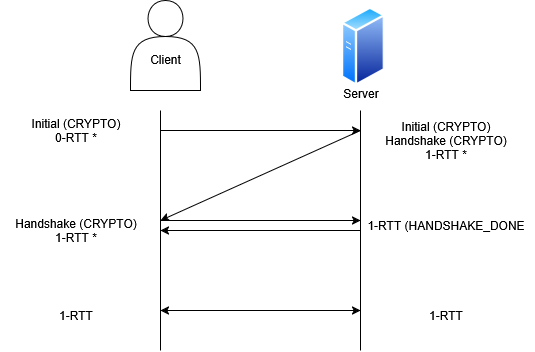
\includegraphics[alt={Diagram of QUIC handshake between a client and a server}, height=9cm]{./images/quic_handshake.png}
	\caption{The QUIC Handshake}
	\label{fig:quic_handshake}
\end{figure}

It is possible to transmit data before the cryptographic handshake has been completed,
albeit with some drawbacks. In Figure~\ref{fig:quic_handshake} the opportunities
for early data transmission have been marked with an asterisk. Firstly, 0-RTT data
transfer is possible, in case the client is previously known to the server and
has received a TLS resumption ticket. With 0-RTT data transfer the initial data may be sent during the Initial Packet
from the client. 0-RTT data transfer comes with the caveat that it is susceptible
to replay attacks. It is also possible for the server to derive the encryption keys
early and transmit data alongside its initial handshake message. This mechanic is
referred to as "0.5-RTT", but the data is carried inside a 1-RTT packet. This has
the drawback of transmitting data before the client has authenticated, which means
that the server should avoid transmitting sensitive data during this transfer. Similarly,
once the client has completed the cryptographic handshake it may already start
transmitting data alongside the TLS Finished message~\cite{rfc9000, rfc9001}.

There are three ways in which a QUIC connection may be terminated. First via an
idle timeout. The idle timeout is configured in the transport parameters, via the
max\_idle\_timeout. If both endpoints announce a max\_idle\_timeout, the lower of
the two will be used. The idle timeout is reset when receiving a packet from the 
peer or alternatively sending a packet to the peer. This means that an endpoint
may defer the idle timeout, by sending a packet to the peer if it expects that
data is still outstanding. If the idle timeout runs out, the connection will be
silently closed, and the state discarded. Second, an endpoint may explicitly
shut down a connection by sending a CONNECTION\_CLOSE frame. This also immediately
closes all open streams, putting the peer that sent the CONNECTION\_CLOSE frame into
the closing state, and the peer that received the CONNECTION\_CLOSE into the draining
state. This is to enable the peers to cleanly shut down their connection and
properly handle packets that arrive out of order. Finally, a connection may be
shut down via a stateless reset. This is used in case the peer does not have
access to the state of the connection, and as a result is unable to process incoming
packets. This causes a Stateless Reset Token to be sent, which is associated with the
connection ID, causing the peer to immediately reset the connection.

\subsubsection{Connection Migration}

The QUIC protocol adds support for connection migration. In legacy protocols such
as TCP, the connection is identified by the tuple pair of source and destination
IP addresses and ports. If something happens that causes any of this information to
change, for example changing from a local network to a mobile network, the connection will
be closed and the state discarded. As discussed in Section~\ref{sec:connections_ids}
one of the motivations for adding connection IDs was to improve the resilience of
connections, allowing the connections to survive changes in network. The connection IDs
are selected by the endpoints, and allow the packets to be correctly routed,
even if the IP address or port of either endpoint changes for any reason~\cite{rfc9000}.

As changes in network port or address may be involuntary, which can happen as a
result from NAT rebinding or a network change, there may be a situation where
either endpoint detects a change to its peer's address or port. The endpoint must then perform
path validation. Path validation is done via sending a PATH\_CHALLENGE frame, containing
a random or hard to guess payload. The peer receives the PATH\_CHALLENGE, and responds
with a PATH\_RESPONSE frame, echoing the payload from the PATH\_CHALLENGE frame.
In this way the path is validated one way. The peer may include its own PATH\_CHALLENGE
frame alongside the PATH\_RESPONCE, to validate reachability the other way~\cite{rfc9000}.

Connection migration may also be initialized explicitly by sending packets from
a new local address. In this case both peers must ensure reachability on the
new path, by using path validation as described earlier in this section. When an endpoint
receives packets from a new address, it must validate the path and subsequently
send packets to the new address, using a new connection ID, to prevent on-wire
tracking of the connection migration. In practice, on the receiving end the process
is the same for explicit and implicit migration. A server will not initialize a 
connection migration, this is exclusively done by the client. What a server may
do is use a preferred address. This allows servers to accept incoming connections
on one address, and then quickly transfer the connection to a separate, preferred
address, performing path validation against the client from the new address~\cite{rfc9000}.

\clearpage

\section{The Server Message Block Protocol}
\label{sec:smb}

The main purpose of the SMB protocol is to share files and directories over a network.
The SMB protocol is a stateful protocol, where clients initiate connections,
an authenticated session is created and requests are sent over the connection, allowing
the client to perform file operations. In addition to sharing files, the SMB protocol enables
access to other network resources, such as printers. There currently exist
two major versions of the SMB protocol, the original SMB protocol, sometimes referred to as the CIFS protocols, which later
evolved into the SMB 2 Protocol, which encapsulates SMB Versions 2 and 3~\cite{smb2_tech}. The SMB 2
protocol will from this point forwards be referred to as the SMB protocol.
The legacy SMB protocol will be referenced as SMB 1 for clarity, however it will
not be covered in depth by this thesis. This section of the thesis will give a
technical overview of the SMB protocol.

Within the larger versions of the SMB protocol there exists minor versions, referred
to as dialects. Within the SMB protocol the following dialects exist, SMB 2,
SMB 2.1, SMB 3.0, SMB 3.0.2 and SMB 3.1.1. The basic functionality of the SMB protocol
was already defined in SMB 1, allowing clients to connect to shares and perform file
operations. As can be seen in the overview given by Table~\ref{tab:smb_dialects},
the protocol has been continuously improved by then, adding support for, among other
features, encryption and alternative transports~\cite{smb2_tech}.

\begin{table}[h]
\centering
\caption{Comparison of SMB protocol dialects}
\label{tab:smb_dialects}
\begin{tabular}{|l|p{5cm}|p{5cm}|}
\hline
\textbf{Dialect} & \textbf{Introduced in} & \textbf{Key Features}\\ \hline
SMB 1.0 & 2000 & Basic file and printer sharing \\ \hline
SMB 2.0 & 2006 & Reduced chattiness, new packet format, support of symbolic links \\ \hline
SMB 2.1 & 2009 & Opportunistic locks, minor performance enhancements \\ \hline
SMB 3.0 & 2012 & Encryption of traffic, multichannel support, SMB Direct (RDMA), transparent failover, Directory Leasing \\ \hline
SMB 3.0.2 & 2013 & Unbuffered read and write \\ \hline
SMB 3.1.1 & 2016 & Support QUIC as a transport, RDMA encryption, Improved cryotography support \\ \hline
\end{tabular}
\end{table}

The SMB protocol places itself in the application layer and it does not stand on its
own but relies on other protocols for much of its functionality. To enable authentication
of clients, the SMB protocol uses the Simple and Protected GSS-API Negotiation (SPNEGO), as
defined in RFC 4178~\cite{rfc4178}. The SPNEGO protocol exposes a common interface
that may be used for authentication with the help of other authentication protocols.
In the case of the SMB protocol the SPNEGO protocols rely on Kerberos Authentication, as
defined in RFC 4120~\cite{rfc4120}, or the New Technology LAN Manager (NTLM) protocol,
as defined in {[MS-NLMP]}~\cite{ntlm_tech} for authentication purposes.

The SMB protocol is designed to be run on top of a reliable transport. Historically
this was NetBIOS over TCP, later standardized to standard TCP. As outlined earlier
in this section, later versions of the SMB protocol support alternative transports. The
SMB dialects >= 3.0 supports use of RDMA via SMB direct, for improved performance.
The latest version of the SMB protocol, 3.1.1 adds support for the QUIC protocol,
which comes with increased security guarantees and potentially improved performance
over TCP~\cite{smb2_tech}.

\subsection{SMB message structure}

The SMB protocol uses the Direct TCP packet header, as shown in Figure~\ref{fig:direct_tcp_header}.
It begins with a zero byte, followed by a 3-byte StreamProtocolLength field which
indicates the length of the SMB2 message. Following this is the actual SMB2 message.
The first part of the SMB2 Message contains the SMB2 packet header. There are 2 versions
of the header, an asynchronous and synchronous header, for asynchronous and synchronous
requests respectively. The first 32 bytes of the SMB2 packet header is common for both
request types, as may be seen from Figure~\ref{fig:smb2_transport_header}. The SMB2 Transport
Header begins with the 4-byte Protocol Id field, which is always set to 0x424D53FE,
or when converted to ASCII and in network byte order, 0xFE, S, M, B. The following field
is the StructureSize, which is set to 64, which is the total size of the header. Next
is the CreditCharge field, this indicates how many credits the request consumes, more on
the SMB credit system later in this chapter. Following this is a field that is 
interpreted differently for the client and the server and depending on dialect.
On the client side, if the dialect is at least SMB 3.0, this field indicates Channel,
for dialects < 3.0, this field is reserved. From the Server side this field indicates
the status in response to any request. The 2-byte command field is used to 
indicate the command of the request or response, Table~\ref{tab:smb_commands} contains
a list of all possible SMB2 commands. Following this is the 2-byte credit request and
response field, which contains information about requested credits. The flags field
contains flags for determining how the packet should be processed. In the SMB
protocol it is possible to concatenate multiple requests into one packet. This is then
indicated via the NextCommand field, that indicates the offset to the next request.
Finally, the MessageId field is the unique identifier that identifies the specific
request and its corresponding response. In addition, the asynchronous header contains
an AsyncId for identifying the asynchronous
operation, a SessionId that identifies the session, and in case the message is signed,
the signature. The synchronous header likewise contains the signature and MessageId, but instead
of the AsyncId the synchronous header contains the TreeId. Following
the SMB2 packet header is the SMB2 Protocol Message, which has a variable length depending
on the command code and if it is a request or a response~\cite{smb2_tech}.

\begin{figure}[h]
	\centering
	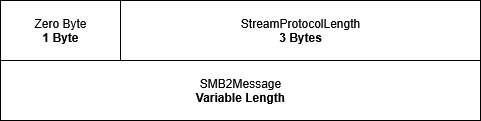
\includegraphics[alt={A block diagram of the SMB Direct TCP header format, detailing its fields and their sizes.}, height=3cm]{./images/smb_tcp_direct_header.drawio.png}
	\caption{The SMB Direct TCP header}
	\label{fig:direct_tcp_header}
\end{figure}

\begin{figure}[h]
	\centering
	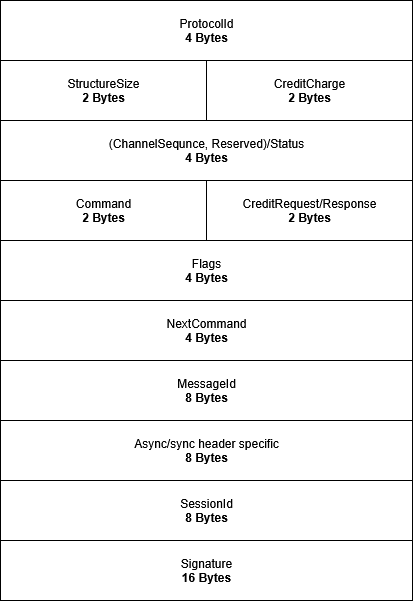
\includegraphics[alt={A block diagram of the SMB2 Packet header common fields format, detailing its fields and their sizes.}, height=14cm]{./images/smb_packet_header_common.png}
	\caption{The SMB protocol header}
	\label{fig:smb2_transport_header}
\end{figure}

\begin{table}[h]
\centering
\caption{SMB Commands}
\label{tab:smb_commands}
\begin{tabular}{|l|l|}
\hline
\textbf{Name} & \textbf{Value}\\ \hline
SMB2 NEGOTIATE & 0x0000 \\ \hline
SMB2 SESSION\_SETUP & 0x0001 \\ \hline
SMB2 LOGOFF & 0x0002 \\ \hline
SMB2 TREE\_CONNECT & 0x0003 \\ \hline
SMB2 TREE\_DISCONNECT & 0x0004 \\ \hline
SMB2 CREATE & 0x0005 \\ \hline
SMB2 CLOSE & 0x0006 \\ \hline
SMB2 FLUSH & 0x0007 \\ \hline
SMB2 READ & 0x0008 \\ \hline
SMB2 WRITE & 0x0009 \\ \hline
SMB2 LOCK & 0x000A \\ \hline
SMB2 IOCTL & 0x000B \\ \hline
SMB2 CANCEL & 0x000C \\ \hline
SMB2 ECHO & 0x000D \\ \hline
SMB2 QUERY\_DIRECTORY & 0x000E \\ \hline
SMB2 CHANGE\_NOTIFY & 0x000F \\ \hline
SMB2 QUERY\_INFO & 0x0010 \\ \hline
SMB2 SET\_INFO & 0x0011 \\ \hline
SMB2 OPLOCK\_BREAK & 0x0012 \\ \hline
SMB2 SERVER\_TO\_CLIENT\_NOTIFICATION (ASYNC only) & 0x0013 \\ \hline
\end{tabular}
\end{table}

\subsection{SMB connection lifetime}

The SMB connection begins by establishing a connection via the transport protocol
of choice. As discussed in Section~\ref{sec:smb}, this may be TCP, RDMA or QUIC.
Once the connection is established, the first message sent from the client is
the SMB2 NEGOTIATE message. The client sends an array of supported dialects,
and in response the server selects the greatest common dialect that is supported
by both parties. In the SMB2 NEGOTIATE response the server also indicates its capabilities,
such as transport encryption in the case of QUIC transport. Once the dialect and
capabilities have been negotiated, the next step in the process is authenticating
the user. This is done via the SMB2 SESSION\_SETUP message. As discussed in Section~\ref{sec:smb},
this is done via the SPNEGO protocol, and the underlying protocol used for authentication
is either NTLM or Kerberos. For Kerberos authentication the client authenticates
against a domain controller, which issues a ticket to the client that can be used for
authentication. In case Kerberos authentication is not available, the client may
authenticate via NTLM. This works by the server sending a challenge to the client,
and using the client password as a shared secret, the response to the challenge is
calculated, and sent back to the server, which verifies the response and authenticates
the client~\cite{smb2_tech}.

Once the SMB connection is established and the client is authenticated, it may now connect
to a share exported by the server. This is done via the SMB2 TREE\_CONNECT request.
The client requests to connect to a specific share, identified with the path name
in the form {\textbackslash\textbackslash}server{\textbackslash}share. The server
tries to find the requested share, and if successful and the client has appropriate
access rights, allocates a specific tree connect object to store information about the session.
This object is identified via a TreeId that is sent back to the client, alongside
the share type: disk, pipe or printer. In addition,
the server returns information about the share capabilities, such as continuous availability
or scaleout capabilities~\cite{smb2_tech}.

Having connected to the share the client is now able to perform the main part of the
transaction, file operations. The client can use SMB2 CREATE to create
or open files, SMB2 CLOSE to close or delete files, SMB2 WRITE and READ to write and
read to and from a file correspondingly, or SMB2 QUERY\_DIRECTORY to list the available files inside
a directory.
Once a file is opened it is identified by an opaque file handle, called an open, returned by the server.
Subsequent file operations are then done via this handle, and the server and client
store the associated information inside a table.
As the SMB protocol is stateful, all the requests are associated with a certain
session, and the requests are handled in accordance with the client's capabilities
and authorization. To limit the number of outstanding requests any client has at
any one time, the SMB protocol uses a credit system. Every
client has a certain number of credits that are consumed upon sending any request.
The number of credits is equal to the size of the request, or the expected size of
the response, whichever is larger, divided by 65536 plus 1. It is up to the client
to request credits as they are consumed, and the server should grant credits when
requested, to avoid a situation where the client reaches 0 credits, as without
any credits the client cannot request any more credits and is then blocked from
performing any more operations~\cite{smb2_tech}.

When the client is finished with a share it is time to disconnect and log off. The
disconnection is performed via a SMB2 TREE\_DISCONNECT message, using the TreeId
provided earlier when connection was set up to the share. If the client is done with its
operations, it can log off from the server via the SMB2 LOGOFF message, allowing
the client to cut all connections to the server. This section only covers the most
basic process and possibilities of using the SMB protocol to access a shared resource.
For further reference the Microsoft Technical documentation~\cite{smb2_tech} outlines all possible
scenarios and is available for further reading into the technical specifics of the
SMB protocol messages and functionalities.

\subsection{SMB over alternative transports}

The SMB protocol currently supports 4 transports, TCP, RDMA, QUIC and the
deprecated TCP over NetBIOS. The standard transport in most scenarios is TCP,
but the protocol is moving towards the use of alternative transports to improve
performance and security. The SMB protocol supports RDMA via SMB Direct. The goal
of RDMA is to allow remote direct memory access, that is reading from and writing
to a remote memory buffer, without having to copy the data. This copy-less operation saves CPU
cycles, and in that way requires less processing power and improves throughput
by using specific network adapters with support for RDMA~\cite{rfc5040}.
The goal of SMB Direct is to improve performance by utilizing RDMA
and multichannel. SMB multichannel allows the client to open multiple transport connections
to the server, improving performance by transferring data in parallel. Encryption over
RDMA is supported since SMB 3.1.1 by encrypting the payloads before they are sent over the
wire~\cite{smb_direct}.

From the perspective of this thesis, the most relevant alternative transport is
SMB over QUIC. As discussed in Section~\ref{sec:quic}, the QUIC protocol brings
many advantages over legacy TCP transports. QUIC enables transport-level encryption
that leverages TLS 1.3 for more secure cryptography, multiple logical streams
to combat HOL blocking, moving the traffic to port 443 to avoid the common port
blocking of SMB port 445 and supports connection migration. The most notable of the improvements to the
SMB protocol is the inclusion of transport level encryption. While SMB version >= 3
supports per share-based encryption, the cryptographic analysis is outside the scope
of this thesis, but benefits of TLS 1.3, such as perfect forward secrecy is not
part of standard SMB encryption~\cite{smb_quic}. SMB over QUIC supports negotiating
transport level encryption in the transport capabilities of the negotiate protocol
request. This allows the client and server to skip SMB level encryption, even though
it is enabled on a share, allowing the communication to rely entirely on QUIC for
securing communications~\cite{smb2_tech}. Additionally, SMB over QUIC supports what is
known as client access control which forces the client to provide its own authentication
via a certificate. As outlined in earlier sections, in TLS 1.3,
during the handshake,  there is the possibility for the server to request that the client
provides its own certificate for authentication purposes. The server can then use
that certificate to determine if the client should be able to connect to the share~\cite{smb_quic_cac}.

\clearpage
\section{Implementing QUIC as transport for SMB server}
\label{sec:implementation}
The QUIC protocol, as outlined in Chapter~\ref{sec:quic}, currently has no kernel
level implementation in Linux, instead relying on user space libraries for support.
This was a conscious design decision for the protocol, allowing for different
implementations and easier iterations as well as switching between different stacks.
There exist many different implementations of QUIC, such as \textit{lsquic} developed by
LiteSpeed, \textit{quiche} developed by Cloudflare and \textit{MsQuic} developed by Microsoft~\cite{quic_implementations}.
There is also an active effort to develop a version of QUIC for the Linux kernel,
driven by Xin Long~\cite{quic_linux_kernel}. For the purposes of this thesis the
MsQuic library was chosen as the library that is used to implement the QUIC transport
layer. The reasoning behind this choice was twofold. Firstly, the MsQuic library
shows promising performance numbers when compared to other libraries~\cite{quic_perf}.
Secondly, as the only SMB over QUIC client currently available is the Microsoft client, it is
advantageous to use the same QUIC implementation both in the server and the client,
to ensure maximum compatibility. This section of the thesis will outline the
architecture and API of the MsQuic library, as well as describe the design of
a QUIC transport layer using the MsQuic library. Additionally the process of integrating
the QUIC transport layer into the Fusion SMB server will be presented.

\subsection{MsQuic architecture and API}
\label{sec:msquic}
The MsQuic library is a cross-platform implementation of the QUIC transport protocol,
implemented as a shared library written in C, with support for development
in C++, Rust and C\#. It is open source and licensed under the MIT-license. The library
utilizes the Windows Secure Channel (Schannel) suite for cryptography functionality
in Windows, and for Linux based OSs the library uses a custom fork of the
OpenSSL library to provide support for QUIC specific cryptography~\cite{msquic}. The
library uses an asynchronous processing model, where the caller creates callback handlers
and registers the handlers with different MsQuic objects, such as listeners and connections.
These callback handlers are then invoked to handle events that occur, such as receiving
a new connection request, a stream being opened or closed, or receiving data on a stream~\cite{msquic_docs}. 

\subsubsection{High level architecture}

\begin{figure}[h]
	\centering
	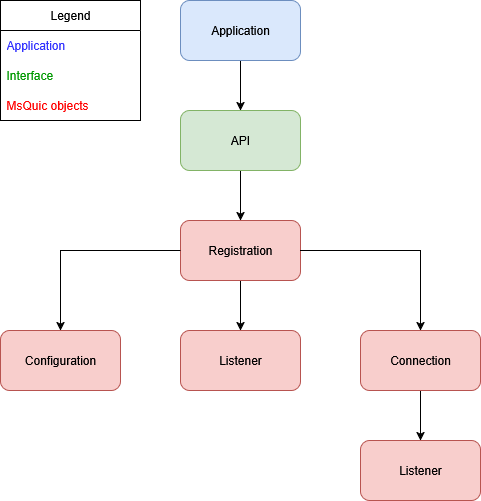
\includegraphics[alt={Block diagram of the high level object model of the MsQuic library, including relationships}, height=11cm]{./images/msquic_architecture.png}
	\caption{High Level MsQuic Object Model}
	\label{fig:msquic_arch}
\end{figure}

The MsQuic library abstracts away the concept of networking sockets, instead opting
for an object-based model, which can be seen in Figure~\ref{fig:msquic_arch}. The
MsQuic library model includes 5 main types of objects: the Registration, Configuration,
Listener, Connection and Stream object. The hierarchy of these objects can be seen
in Figure~\ref{fig:msquic_arch}. All function calls are done in relation to one of
these objects with the exception of the call to initialize the library, which returns
a function table of MsQuic functions, and the corresponding call to close the library~\cite{msquic_docs}.

The Registration object represents the execution context for the transport, being
responsible for the connection logic and creating the threads that are used for
processing. All other objects are created under the registration, and each registration
is completely independent from one another, with resources and scope being
unique to each registration. In practice this means that one application generally
uses only one registration~\cite{msquic_docs}.

The configuration object stores the settings that are used in configuring the MsQuic
library. These include the QUIC transport settings, as well as security configurations. Everything
from initial receive windows, idle timeout timers to the congestion algorithm used
can be configured. The comprehensive list of configuration parameters can be found
in the MsQuic documentation. In addition, each of the MsQuic objects have specific
parameters that can be configured, and the certificate as well as its parameters
is separately configured, for example configuring requesting a certificate from the client
and allowed cipher suites. The configuration object also stores a list of
Application Layer Protocol Negotiation (ALPN) IDs that the server supports~\cite{msquic_docs}.
ALPN is a TLS feature, that is designed for a situation where it is not clear which
service a client is trying to access. This may arise when a server is running
multiple network services that all use the same port, for example the SMB over
QUIC protocol uses the same UDP
port as HTTP/3. ALPN allows the server and client to negotiate which protocol
will be used inside the TLS tunnel, removing the need for an additional round trip to negotiate
the used protocol separately~\cite{rfc7301}. For reference SMB over QUIC simply uses the ALPN ID "smb".

The listener object is responsible for listening for
and accepting incoming connections. The listener object uses a callback function
that is responsible for handling incoming connections. The callback function decides
if the incoming connections is accepted, and if it is a connection object is created
in response~\cite{msquic_docs}.

The Connection object represents the QUIC connection between two peers. On the client
side this connection is explicitly created via a function call, while on the server
side it is created in the listener callback. The connection object contains information
about the connection, and it is expected to handle events related to connection set up,
stream creation and connection teardown, either as a result of an error or from one
of the peers closing the connection~\cite{msquic_docs}.

The most important object type is the Stream object, as it is responsible for
the data transfer between the peers. As discussed in Section~\ref{sec:quic}, there
can be a theoretical unlimited number of streams on top of a connection, but in
practice the maximum number is configured in the MsQuic library, with separate
limits for unidirectional and bidirectional streams. New streams can be created
either by the client or the server, with the other party being notified of
the event. When sending data the MsQuic library takes temporary ownership of the
buffer, copying the data internally and queuing the data to be sent. This allows
the MsQuic library to pace the sending and "keep the pipe full", aiming to not let
the stream sit unnecessarily idle. It is also possible to disable this internal buffering,
instead making the caller responsible for queuing enough sends to prevent idling
the connection~\cite{msquic_docs}.

Receiving data happens via a receive event, that gets passed to the callback function.
This includes references to buffers that contain the received data. The data can
then either be processed inside the callback or passed along to a separate
thread to be processed. Either way, the caller needs to signal to the library when
the data has been processed, giving back ownership of the buffers to the library. This
also indicates that the caller is ready to receive more data. Normally only one receive
event can be active at one time, i.e. the library will not indicate that more data is
available before the application has signaled that the previous set of data has been processed.
Alternatively, the MsQuic library supports Multi-receive mode,
where the library will keep creating receive events when data is available, and
it is up to the caller to keep track of the number of bytes processed, and report
this back to the library. This enables more efficient processing of data when the
processing is done asynchronously in a separate thread~\cite{msquic_docs}.

\subsection{Fusion SMB server QUIC transport layer design}

As discussed in earlier section, network communication using TCP experiences
some drawbacks related to the fundamental design of the protocol, drawbacks
which the QUIC protocol aims to solve. This section describes the design of a
QUIC transport layer for the Fusion SMB server, utilizing the MsQuic library for
implementing QUIC functionality. The decision to use the MsQuic library was discussed
earlier in Section~\ref{sec:implementation}. The main goal of this project is to create
a QUIC transport layer that supports all the necessary QUIC features such that it
is able to communicate with and establish a connection with the Microsoft SMB over
QUIC client. A secondary goal is to design the QUIC transport layer in such a way
that the performance, measured via throughput during various workloads, is comparable
to the standard SMB stack using TCP on an encrypted share. This allows the QUIC transport
layer to work as an improvement to the standard TCP transport layer, with improved
security via TLS 1.3, resilience to SMB port blocking from ISPs and connection migration
support, relevant especially for mobile users.

\subsubsection{MsQuic Integration into Fusion SMB}

The generic transport layer interface of the Fusion SMB server uses a set of functions
that is called by the server to interact with the transport, such as for creating and
destroying the transport, listening for incoming connection and receiving and transmitting data.
This requires a little bit of work around when integrating with the MsQuic library, as
it does not conform to standard BSD-style socket semantics. Figure~\ref{fig:msquic_int}
gives a high-level overview of the interface between the QUIC transport layer and the
rest of the server. The processing begins by creating the specific transport, which
is configured inside the Fusion SMB configuration. This causes the server to create
one of two new types of transport, IPV4\_QUIC or IPV6\_QUIC. During the creation the MsQuic
library is initialized, and the specific configuration options are read in and stored,
such as listening interface and TLS credentials, which are needed later. A listener
object is created and starts listening for incoming connections. When a connection
arrives via a QUIC\_LISTENER\_EVENT\_NEW\_CONNECTION event, the listener accepts the
connection and passes it along to the
connection callback handler. The connection callback continues the handshake by using the TLS
credentials stored earlier and creates an internal connection object storing
the connection information that is necessary for the protocol. This internal connection
object is passed back to the Fusion SMB server, that stores the connection internally
as an active connection. The connection is now set up, and the connection object continues waiting
until a QUIC\_CONNECTION\_EVENT\_PEER\_STREAM\_STARTED event arrives, indicating
that a new stream, with associated data has been opened. This causes a stream object
to be created, with its associated callback function set. The stream object works
as a middle layer between the Fusion SMB server and the QUIC transport, receiving
data into a receive buffer for the server, and transmitting data from the server to
the client, enabling two-way communication between the server and client.

\begin{figure}[h]
	\centering
	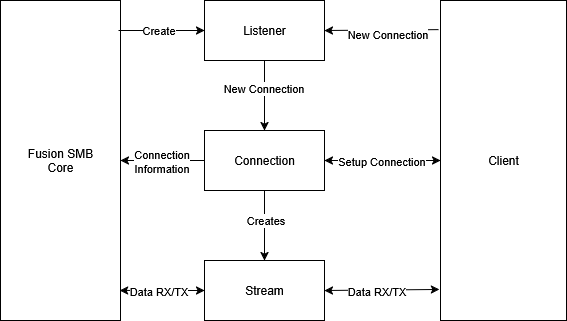
\includegraphics[alt={Block diagram of the flow between Fusion SMB and MsQuic}, height=12cm]{./images/MsQuic_integration.png}
	\caption{MsQuic integration with Fusion SMB}
	\label{fig:msquic_int}
\end{figure}

\subsubsection{QUIC transport layer data path}

When implementing the QUIC layer, the multi-receive mode of the MsQuic
library, as outlined in Section~\ref{sec:msquic}, will be used due to the improved performance
this offers the application. In practice this means that as soon as data is available,
the stream callback is invoked with a QUIC\_STREAM\_EVENT\_RECEIVE event, containing
the received data. This data should then be processed in a separate thread, that is not in
the callback handler inside the MsQuic worker thread. This is accomplished by passing
along the data to the Fusion SMB server's internal threads. To enable this,
when data is received, the reference to the received buffers is copied into a separate
data structure, as seen in Figure~\ref{fig:msquic_buf}, consisting of a linked list
of buffers. This choice was made as it cannot be guaranteed that the servers is able to drain 
the incoming data faster than it arrives, and the linked list structure allows
the total buffer size to grow dynamically as needed. This method of handling incoming
network buffers is similar to the method used in the Linux kernel, albeit a simplified
version, using a single-linked list instead as compared to the doubly linked list
used in the Linux kernel~\cite{linux_network_buffer}.
As can be seen in Figure~\ref{fig:msquic_rx_data} the data is not copied until
it reaches the internal receiving thread, with only the reference to the received buffer being
passed around. This allows the processing in the callback function to be inexpensive,
quickly freeing up the worker thread for additional processing.
This solution of storing the received buffer temporarily in a linked list simplifies
integration with the existing receive interface, as the receiving threads
expect BSD-style socket semantics, that is issuing read calls to read in data, instead of the
event driven model that is used by the MsQuic library. The linked list then works as a middle
layer, allowing the receive interface to work with the QUIC transport layer without modification.
When draining the receive buffer the caller begins from the head, reading in as
much data as necessary, updating the offset, and if the head is completely drained,
moves onto the next element in the list, until the requested amount of data has
been drained.

\begin{figure}[h]
	\centering
	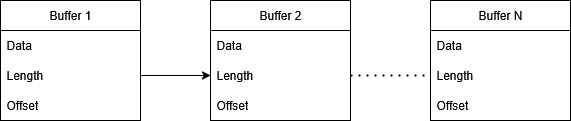
\includegraphics[alt={Block diagram of the receive buffer of the QUIC layer}, height=3cm]{./images/quic_buffer.png}
	\caption{QUIC transport layer receive buffer}
	\label{fig:msquic_buf}
\end{figure}

\begin{figure}[h]
	\centering
	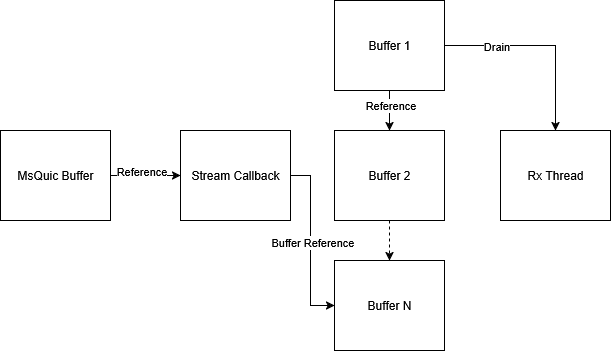
\includegraphics[alt={Block diagram of how the buffer moves from MsQuic to RX thread}, height=8cm]{./images/rx_buf_flow.png}
	\caption{Data flow from MsQuic buffer to RX thread}
	\label{fig:msquic_rx_data}
\end{figure}

The steps of receiving data and getting it into the Fusion SMB core can be seen in Figure~\ref{fig:msquic_rx}.
When data has arrived, and the buffer information has been copied into the receive buffer list, the
next step is checking if the buffer is currently actively being drained. If it is,
the callback signals to the draining thread that there is more data available to be read. Otherwise,
the callback sends an internal IPC message to the receiving threads, signaling that there is data available
on this connection and for a receiver thread to start processing. From the callback function
STATUS\_PENDING is returned to the MsQuic library, signaling that the data is being
processed in a separate thread. Once the receiving thread has finished draining the buffers,
it calls StreamReceiveComplete() with the number of bytes drained, signaling to the
MsQuic library that the processing of the received data is at least partially complete. 
\begin{figure}[h]
	\centering
	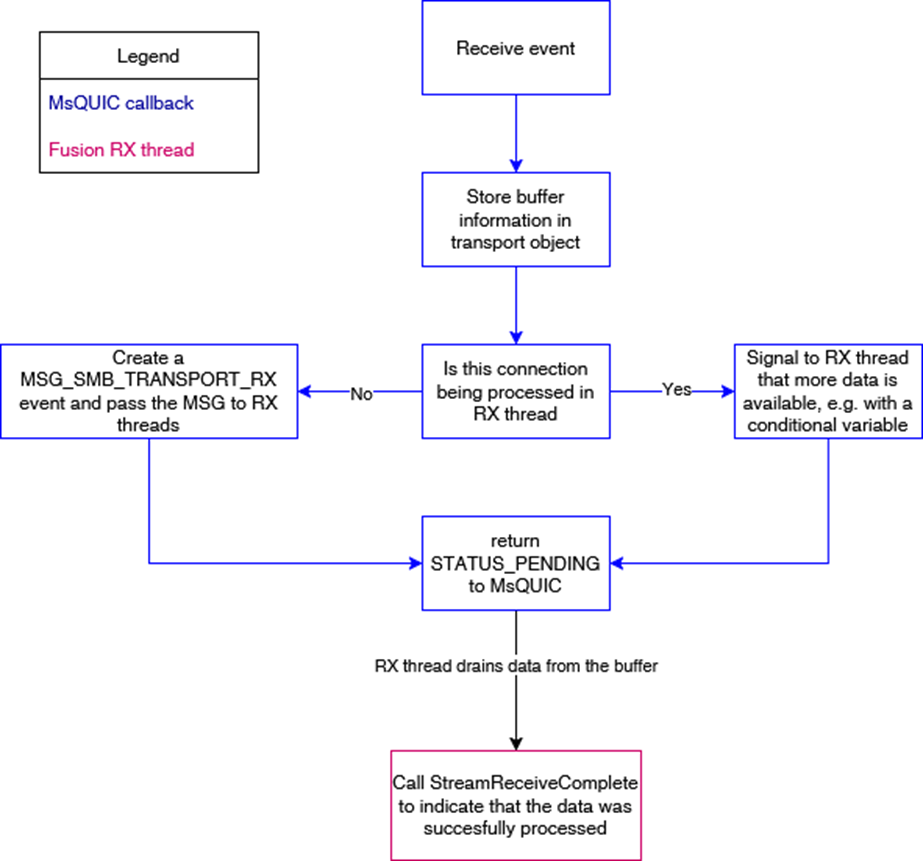
\includegraphics[alt={Block diagram of the flow when receiving data using the MsQuic library}, height=13cm]{./images/receive_flow.png}
	\caption{QUIC transport layer receive flow}
	\label{fig:msquic_rx}
\end{figure}

The transmission of data is less involved than receiving data, as can be seen
in Figure~\ref{fig:msquic_tx}. When data is to be transmitted it is stored in
an array of buffers in the iovec format\footnote{\url{https://man7.org/linux/man-pages/man3/iovec.3type.html}}. When transmitting the data the MsQuic
library expects the buffers to be in its own internal QUIC\_BUFFER format,
so the iovecs could simply be cast to the QUIC\_BUFFER struct. However, as the MsQuic call to transmit
data, StreamSend(), is non-blocking, it is not guaranteed that by the time the buffers
are freed in the transmitting thread, that the MsQuic library has had time to transmit them yet.
So, to simplify lifetime tracking of the buffers we instead copy them into new QUIC\_BUFFERS,
adding one additional copy.
The original buffers are freed as soon as the StreamSend() call returns, while the new
buffers get freed in the callback handler once transmission is complete, as signaled by a STREAM\_SEND\_COMPLETE
event in the MsQuic stream callback thread.

Testing against Microsoft's SMB over QUIC client shows that the client utilizes the
QUIC transport in the same way that it would use a TCP transport, that is it only
open a single stream per connection. This greatly simplifies processing of received
and transmitted data, as there is no need to track an arbitrary number of streams
per connection.

\begin{figure}[h]
	\centering
	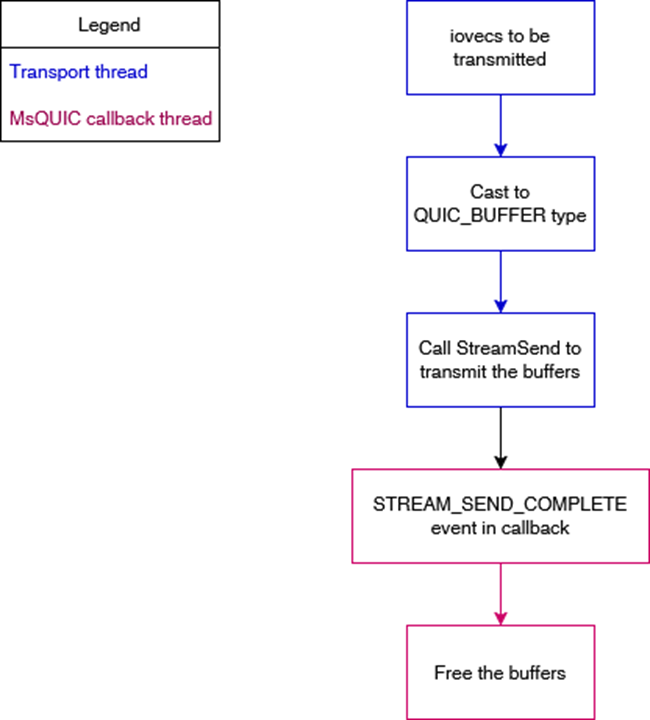
\includegraphics[alt={Block diagram of the flow when sending data using the MsQuic library}, height=13cm]{./images/send_flow.png}
	\caption{QUIC transport layer transmission flow}
	\label{fig:msquic_tx}
\end{figure}

\clearpage
\section{Benchmarking}
\label{sec:benchmark}
\subsection{Test environment}

\paragraph{Hardware environment}

As illustrated in Figure~\ref{fig:hardware} the hardware environment for the test setup consists
of a server and a client, connected directly via a 100 GbE switch. The server is a Supermicro
SYS-2029BT-HNR, with dual Intel Xeon Gold 622R CPUs running at a clock speed of 2.9 GHz. The server
has 192 GB of RAM, and a 3 TB Micron 9300 NVMe drive supporting read and write speeds of 3.5 GB. The client
machine is a Gigabyte R281-3C1, with dual Intel Xeon Silver 4114 CPUs, running at a clock speed of 2.2GHz.
Similarly to the server the client has 192 GB of RAM.

\begin{figure}[h]
	\centering
	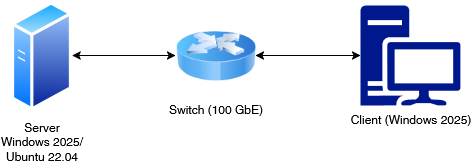
\includegraphics[alt={Block diagram of hardware setup of test environment}, height=4cm]{./images/hardware.png}
	\caption{Test environment hardware setup}
	\label{fig:hardware}
\end{figure}

\paragraph{Software environment}

The server is set up to dual boot Windows 2025 and Ubuntu 22.04 LTS, allowing for the benchmarks to
be run against the same hardware for both the Fusion SMB and Windows SMB implementations. The
client is running Windows 2025 to support SMB over QUIC client capabilities.

\subsubsection{SMB over QUIC implementations analyzed}
As part of this thesis two different SMB over QUIC implementations were considered
for comparison in the benchmark.

\paragraph{Fusion SMB server:}

The Fusion SMB server, with the prototype QUIC transport layer as described in
Chapter~\ref{sec:implementation}, will be the first item of comparison. The performance
of the Fusion SMB server with the MsQuic library for QUIC transport capabilities will
be compared to the Windows SMB over QUIC implementation, as well as the traditional
TCP-based transport.

\paragraph{Windows SMB over QUIC server:}

The Windows SMB over QUIC server implementation provided by Microsoft is currently
the only production-ready and widely deployed implementation of SMB over QUIC. The
Windows server will be the main target of comparison
against Fusion SMB, comparing the direct performance of QUIC as well as the performance
impact of using QUIC in place of TCP for SMB traffic.

\paragraph{Windows SMB over QUIC client:}

The Windows SMB over QUIC client provided by Microsoft is, as with the server implementation,
the only production-ready and widely deployed implementation of SMB over QUIC. The client
will be used for testing both against Fusion SMB and Windows SMB server.

\subsubsection{Benchmarking Software}

For measuring the link speed and making sure the tests are running over the correct
network interface, iPerf\footnote{\url{https://iperf.fr/}} will be used. iPerf allows
for the testing of the maximum bandwidth over a network, and will indicate any
possible issues or bottlenecks in the test environment.
The MsQuic repository contains a tool for testing the performance of MsQuic called
SecNetPerf\footnote{\url{https://github.com/microsoft/msquic/tree/main/src/perf}},
which implements a QUIC performance protocol defined in~\cite{banks-quic-performance-00}.
The tool enables the testing of link throughput, which means that the tool is used
to get a baseline performance of MsQuic over the link used for testing. This value can then
be compared to the throughput of the SMB over QUIC solution, to determine the overhead
introduced by the implementation of the QUIC transport layer together with the SMB protocol.

To ensure reproducibility and comparability of the results, filesystem benchmarks are run
using the Flexible I/O (fio) tester \footnote{\url{https://fio.readthedocs.io/en/latest/fio_doc.html}},
which enables running synthetic workloads on the shares. The fio tester supports
many different scenarios, workloads as well as fine-grained control over parameters
such as file and block size, sequential and random reads as well as time-based workloads.

\subsection{Test scenarios}

\subsubsection{Interoperability tests}

The first step in testing, before performance evaluation, is to make sure that
the two implementations outlined are able to connect, authenticate and set up
the SMB session. Using the Windows SMB over QUIC client, it is ensured that the client
is able to connect to the server, receive and accept the server certificate, and
additionally perform some basic file operations to ensure that the data transfer is
working properly. Additionally, the connection should remain stable during the lifetime
of the connection, and teardown should be handled gracefully.

\subsubsection{Benchmarking scenarios}

The exact commands used in running the benchmarks are available in Appendix~\ref{app:bench}.
The tests were chosen in such a way as to both benchmark the solutions under optimal conditions,
as well as represent real world scenarios. The FIO benchmarks were all run for a time of
120 seconds to ensure that the results would represent an average throughput under sustained
load and minimize the impact of external conditions.

\paragraph{iPerf:}
iPerf is run using the standard setup, with no additional parameters. This benchmark tests
the maximum possible network throughput during a time period of 10 seconds.

\paragraph{SecNetPerf:}
For running the SecNetPerf performance test to get an overview of the link speed,
two tests are run, one for checking the link speed each way. The test is run with the maximum
throughput execution profile, and runs for 60 seconds, first testing uplink speed,
then downlink speed (from the perspective of the client). This gives a base value for
what the optimal throughput is expected to be, as logically the addition of the
overhead of QUIC transport layer, SMB protocol and filesystem IO should not improve
performance. This test also should work as a check that the environment is correctly
set up, as unexpected results may point to problems in the configuration.

\paragraph{FIO Scenario 1: Sequential read and write of single large file}

The sequential read and write of one file is used to establish baseline numbers
for the performance of the transport. The test is designed such that it puts little
strain on the filesystem IO, instead of having the transport layer as the primary 
bottleneck for performance. The tests are run against a
pre-allocated 5GB file, allowing for a maximum throughput test during continuous load.
This test uses a large block size to maximize the performance.

\paragraph{FIO Scenario 2: Random read and writes of a single large file}

In comparison to scenario 1, where the maximum throughput is tested, scenario 2
with random reads and writes instead tests the performance when there is a lot of
small operations. The main performance metric of scenario 2 is the number of I/O operations per second (IOPS).
To simulate this workload, it is run against a 1 GB file, with a small blocksize
together with random writes and reads. This corresponds
to workloads where many small operations are done consistently, for example in
spreadsheets.

\paragraph{FIO Scenario 3: Read and write of many small files}

The final FIO scenario is the reading and writing of many small files concurrently,
testing workloads where there is a lot of concurrency. The test creates 16 files
of size 100 kB and performs random reads and writes against the files. This allows the benchmarking
of a scenario with many processes simultaneously performing workloads, stress
testing different parts of the processing than scenario 1 and 2.

\subsection{Results}

This section will outline the results from the benchmarks outlined in Section~\ref{sec:benchmark}.
For each of the scenarios there are two sets of graphs, one outlining the IO performance
in MB/s, as well as the IOPS. As the benchmarks used consistent block sizes, it is
expected that these two metrics are heavily correlated. Each of the scenarios were
run against SMB over QUIC,
as well as against SMB using TCP. The QUIC benchmarks were ran against an unencrypted
share, instead relying on the QUIC protocol's integrated encryption. The TCP benchmarks
were run against an encrypted SMB share, so that the performance numbers would be
comparable with the performance number from SMB over QUIC.
\begin{figure}[h]
\centering
\begin{tikzpicture}
\begin{axis}[
    ybar,
    enlargelimits=0.10,
	enlarge y limits={upper=0},
    legend style={at={(0.5,-0.15)},
      anchor=north,legend columns=-1},
	ylabel=Throughput (Gb/s),
	symbolic x coords={iPerf, Secnetperf up, Secnetperf down},
    xtick=data,
	ymin=0
    ]
\addplot 
	coordinates {(iPerf,13.400) (Secnetperf up, 3.900) (Secnetperf down, 3.200)};

\addplot 
	coordinates {(iPerf,20.000) (Secnetperf up, 6.100) (Secnetperf down, 3.100)};
\legend{Windows, Ubuntu}
\end{axis}
\end{tikzpicture}
\caption{Link speed throughput}
\label{fig:perf_graph}
\end{figure}

As can be seen in Figure~\ref{fig:perf_graph}, the link speed was verified using both
iPerf and SecNetPerf. The performance tests were run using the Windows 2025 client
machine as the performance test client, against both the Windows and Ubuntu
server hosts. Using the default settings of iPerf, the throughput reached 20 Gb/s
against the Ubuntu host, and 13.4 Gb/s against Windows. Similarly, using SecNetPerf,
speeds of at least 3 Gb/s where reached both ways, for both servers. This indicates
that under optimal conditions, a single QUIC connection and stream using MsQuic can at most reach
speeds of 3Gb/s on the test hardware, indicating the point where the throughput is limited by the MsQuic
library.

The interoperability of the SMB over QUIC implementation, as outlined in Chapter~\ref{sec:implementation},
was manually tested using the Windows 2025 SMB over QUIC client. This was accomplished
by using PowerShell to mount the share. By specifying \textit{/transport:quic} when
mounting the share, it is possible to force the client to exclusively try to connect
via QUIC, completely forgoing TCP. A self-signed certificate was used in the server
for testing purposes, and the client was configured to accept the certificate by
specifying \textit{/skipcertcheck} when mounting the share. Via manual testing it
was shown that the client could mount the share, create a text file, write some
data to the file, delete the file and finally disconnect from the server, without
any issues. This showed that the compatibility aspect of the implementation had been
reached.

\subsubsection{Scenario 1: Large sequential I/O}
\begin{figure}[h]
\centering
\begin{tikzpicture}
\begin{axis}[
    ybar,
    enlargelimits=0.25,
	enlarge y limits={upper=0},
    legend style={at={(0.5,-0.15)},
      anchor=north,legend columns=-1},
	ylabel=Throughput (MB/s),
	symbolic x coords={Read, Write},
    xtick=data,
	ymin=0
    ]
\addplot 
	coordinates {(Write,432) (Read, 337)};
\addplot 
	coordinates {(Write,457) (Read, 623)};
\addplot 
	coordinates {(Write,663) (Read, 727)};
\addplot 
	coordinates {(Write,1319) (Read, 566)};
\legend{Fusion(QUIC), Windows(QUIC), Fusion(TCP), Windows(TCP)}
\end{axis}
\end{tikzpicture}

\begin{tikzpicture}
\begin{axis}[
    ybar,
    enlargelimits=0.25,
	enlarge y limits={upper=0},
    legend style={at={(0.5,-0.15)},
      anchor=north,legend columns=-1},
	ylabel=IOPS,
	symbolic x coords={Read, Write},
    xtick=data,
	ymin=0
    ]
\addplot 
	coordinates {(Write,412) (Read, 321)};
\addplot 
	coordinates {(Write,435) (Read, 594)};
\addplot 
	coordinates {(Write,632) (Read, 693)};
\addplot 
	coordinates {(Write,1257) (Read, 539)};
\legend{Fusion(QUIC), Windows(QUIC), Fusion(TCP), Windows(TCP)}
\end{axis}
\end{tikzpicture}
\caption{Scenario 1 results: Large sequential I/O}
\label{fig:scenario_1}
\end{figure}

The results of benchmark scenario 1 are outlined in Figure~\ref{fig:scenario_1}.
Looking at the write workloads it can be seen from the graphs that there is
one significant outlier, the throughput of the write workload from the Windows Client
to the Windows server using encrypted TCP.
The reason for this outlier is not evident, the gain could potentially be from offloading
of cryptographic processing to a separate thread or some other optimization in the
threading model of the implementation. 
Due to this outlier the Windows SMB over QUIC implementation suffers a 65\%
performance reduction when compared to encrypted TCP. In comparison, the Fusion QUIC
transport prototype sees a 35\% reduction in throughput for the write workload when compared
to encrypted TCP. For the read
workload the Windows QUIC implementation actually performed slightly better than
using encrypted TCP, while the Fusion QUIC implementation sees a 50\% reduction in
throughput as compared to encrypted TCP, suggesting that there are optimizations
that could be made to the transmitting data path in the QUIC prototype, to bring
the comparative performance in line with the read throughput. This is also evident
when comparing Windows QUIC performance with Fusion QUIC performance. The write
workload, which is mainly bounded by the client's performance, shows very similar performance between
both QUIC implementations. In comparison, the read workload, which is more dependent
on the server, shows that the Fusion QUIC implementation has a 45\% lower throughput than
the Windows QUIC implementation.

\subsubsection{Scenario 2: Single file random I/O}

\begin{figure}[h]
\centering
\begin{tikzpicture}
\begin{axis}[
    ybar,
    enlargelimits=0.25,
	enlarge y limits={upper=0},
    legend style={at={(0.5,-0.15)},
      anchor=north,legend columns=-1},
	ylabel=Throughput (MB/s),
	symbolic x coords={Read, Write},
    xtick=data,
	ymin=0
    ]
\addplot 
	coordinates {(Write,130) (Read, 143)};
\addplot 
	coordinates {(Write,170) (Read, 147)};
\addplot 
	coordinates {(Write,140) (Read, 140)};
\addplot 
	coordinates {(Write,216) (Read, 141)};
\legend{Fusion(QUIC), Windows(QUIC), Fusion(TCP), Windows(TCP)}
\end{axis}
\end{tikzpicture}

\begin{tikzpicture}
\begin{axis}[
    ybar,
    enlargelimits=0.25,
	enlarge y limits={upper=0},
    legend style={at={(0.5,-0.15)},
      anchor=north,legend columns=-1},
	ylabel=IOPS,
	symbolic x coords={Read, Write},
    xtick=data,
	ymin=0
    ]
\addplot 
	coordinates {(Write,31800) (Read, 34900)};
\addplot 
	coordinates {(Write,41500) (Read, 35800)};
\addplot 
	coordinates {(Write,34300) (Read, 34200)};
\addplot 
	coordinates {(Write,52700) (Read, 34400)};
\legend{Fusion(QUIC), Windows(QUIC), Fusion(TCP), Windows(TCP)}
\end{axis}
\end{tikzpicture}
\caption{Scenario 2 results: single file random I/O}
\label{fig:scenario_2}
\end{figure}

Scenario 2, in comparison to scenario 1, shows much less impact from the different
transports, which can be seen in Figure~\ref{fig:scenario_2}. For the read workload it is
clear that the difference in results is insignificant, with all transports and hosts
showing very similar throughput, for both QUIC and encrypted TCP. In the case of the write workload it can be seen
that as in scenario 1, the Windows server shows a higher throughput, and the difference
between QUIC and encrypted TCP is significant for the Windows implementation. Again, the
Windows QUIC implementation has slightly higher throughput than the Fusion QUIC implementation,
but the difference is less severe than in Scenario 1, with the Fusion QUIC implementation
suffering a 30\% decrease in throughput. From Scenario 2, it can be seen that the bottleneck is
not only the network transport layer, resulting in similar performance regardless
if QUIC or encrypted TCP is used.

\subsubsection{Scenario 3: multiple files random I/O}
\begin{figure}[h]
\centering
\begin{tikzpicture}
\begin{axis}[
    ybar,
    enlargelimits=0.25,
	enlarge y limits={upper=0},
    legend style={at={(0.5,-0.15)},
      anchor=north,legend columns=-1},
	ylabel=Throughput (MB/s),
	symbolic x coords={Read, Write},
    xtick=data,
	ymin=0
    ]
\addplot 
	coordinates {(Write,46) (Read, 44)};
\addplot 
	coordinates {(Write,48) (Read, 41)};
\addplot 
	coordinates {(Write,57) (Read, 53)};
\addplot 
	coordinates {(Write,85) (Read, 79)};
\legend{Fusion(QUIC), Windows(QUIC), Fusion(TCP), Windows(TCP)}
\end{axis}
\end{tikzpicture}

\begin{tikzpicture}
\begin{axis}[
    ybar,
    enlargelimits=0.25,
	enlarge y limits={upper=0},
    legend style={at={(0.5,-0.15)},
      anchor=north,legend columns=-1},
	ylabel=IOPS,
	symbolic x coords={Read, Write},
    xtick=data,
	ymin=0
    ]
\addplot 
	coordinates {(Write,11200) (Read, 10800)};
\addplot 
	coordinates {(Write,11700) (Read, 9600)};
\addplot 
	coordinates {(Write,13900) (Read, 12900)};
\addplot 
	coordinates {(Write,20900) (Read, 20200)};
\legend{Fusion(QUIC), Windows(QUIC), Fusion(TCP), Windows(TCP)}
\end{axis}
\end{tikzpicture}
\caption{Scenario 3 results: multiple files random I/O}
\label{fig:scenario_3}
\end{figure}

Scenario 3, illustrated in Figure~\ref{fig:scenario_3}, shows that
Windows using encrypted TCP has a significant advantage in this scenario, when compared
to the other implementations. This advantage holds for both for read and write workloads.
However, when comparing the performance of SMB over QUIC, the
throughput of Windows and Fusion is very close, with Fusion being slightly favored
in the read workload, and Windows having a slight advantage in the write workload.
The throughput of Fusion's implementation of QUIC and encrypted TCP is close, just as
in scenario 2. In comparison, the performance impact of using QUIC instead of
encrypted TCP is more significant for the Windows implementation, which can be seen
in the results of all three scenarios.

\clearpage
\section{Conclusions}
\label{sec:conclusion}
\label{sec:summary}

This thesis has explored the feasibility of implementing SMB on top of QUIC,
and a prototype SMB over QUIC implementation has been created. Due to the fact that the
Windows SMB over QUIC client and server implementation only uses one stream per connection, the semantics of
SMB over QUIC is very similar to that of the traditional TCP-based implementation,
making it very feasible to implement SMB on top of QUIC.
The biggest hurdle in implementing SMB over QUIC is the lack of native QUIC support in Linux-based
systems, necessitating the use of external libraries to provide support for the QUIC protocol.
The external library chosen for the implementation, MsQuic, differs in processing model
and interface from standard BSD-style sockets, leading to the design and work needed to integrate
the QUIC layer being non-trivial.

The biggest benefits of using a QUIC-based SMB implementation as compared to the TCP-based implementation
is the improved cryptography of TLS 1.3 and the move from TCP port 445, which is commonly
blocked by ISPs, to UDP port 443, which is also used by HTTP/3, enabling the SMB
traffic to traverse the internet without getting blocked. The biggest disadvantage is
the negative performance impact of using QUIC as compared to TCP in high-throughput
scenarios.

During the process of this thesis, two SMB over QUIC implementations have been benchmarked
during optimal network conditions, and the results have been presented. Additionally,
the same benchmarks were run against SMB over encrypted TCP, and the performance of SMB
using TCP and QUIC was compared. The benchmarks show that during optimal network conditions
the QUIC-based implementations' performance suffers when compared to TCP-based implementations,
but the performance numbers from the QUIC-based implementations are promising and
the performance is already sufficient for general-purpose tasks. The rest of this section of the
thesis will summarize the key points and findings of the thesis
and add some discussion about the possible expansions of SMB over QUIC.

\subsection{Discussion}

This work has been successful in designing and implementing a prototype QUIC transport layer
for the Fusion SMB server to provide SMB over QUIC functionality.
While the prototype's performance somewhat suffers in scenarios that are heavily dependent
on the network transport throughput, the Fusion SMB over QUIC implementation still managed to
nearly match the performance of encrypted TCP for workloads that are not only dependent
on the network transport performance. The prototype is a promising first step in implementing an SMB over QUIC
implementation for Linux based systems.

While there is room for improvements in the performance of the QUIC transport layer,
the implemented prototype still shows relatively good performance. While under ideal
conditions the QUIC transport layer suffers when compared to encrypted TCP, it must be highlighted
that one of the main advantages of SMB over QUIC is the ability to access SMB shares from
external networks, as compared to legacy SMB access which is most commonly
done inside internal networks or over Virtual Private Networks (VPN). This is since
that the standard SMB TCP port 445 is commonly blocked by ISPs, affecting the ability
of SMB traffic to traverse the internet. Considering that
most ISPs only offer internet bandwidths of up to 1 Gb/s (125 MB/s), the prototype is
already able to sufficiently support access over the internet.

During the process of working on this thesis it became clear that the extensions
to the SMB protocol made by Microsoft to support SMB over QUIC were done in such a way
that they do not take advantage of many of the improvements offered by QUIC when compared
to TCP. There are only two QUIC specific features utilized by SMB. First, transport level
encryption with the SMB protocol, moving the encryption from an SMB specific per-share basis to
instead use QUIC's native encryption. Second, SMB over QUIC implements mutual
authentication, allowing authentication of clients via certificates. However, there is
at least one significant QUIC feature missing, from
the [MS-SMB2] documentation \textit{"By default, Windows SMB2 clients and servers always use a single stream per QUIC connection.
Sending or receiving more than one stream per connection will be blocked by the underlying transport
QUIC."}~\cite{smb2}. This, in turn, results in the SMB protocol entirely neglecting
to use one of the biggest improvements brought on by QUIC, the ability to use
multiple data streams over one connection. The following are some of the author's suggestions
on how the SMB protocol could properly implement support for QUIC and its
modern features.

As QUIC streams are by design lightweight, the overhead of opening new streams,
when compared to for example the overhead introduced by filesystem I/O, is
negligible. The main drawback to implementing a system of multiple streams per
connection is the increased complexity, as there are no guarantees of in-order
delivery between the streams. A server or client might transmit two streams, one after the
other, and they may arrive in the reverse order. However, the SMB protocol already
has added support for SMB Multichannel, which enables the server and client to transmit
and receive over multiple Network Interface Controllers (NIC), or utilize multiple
paths over one NIC via Receive Side Scaling (RSS), simultaneously. Thus, the problem
of data transfer over multiple data streams has already been solved via earlier
extensions to the protocol.

The main issue is then working out how multiple requests should be split up between different
streams, and what the granularity of these splits could be. The naive approach
is to map every request or compounded request to its own stream. One stream would then
consist of a request and a response, or a set of compounded requests and compounded
responses. This is similar to the design of HTTP/3 or DNS over QUIC. The advantage
of this approach is that it takes full advantage of
the multiplexed streams implemented by QUIC, going a long way towards negating HOL blocking.
Another approach is to use streams on a per-open basis, setting up a stream
for each file or directory that is opened, and sending all operations concerning that file
or directory over its specific stream. The advantage here is lesser complexity than having
all requests on separate streams, while still managing to take advantage of QUIC's advanced
features.

There are some other advantages that may be implemented regardless of how the requests
are split between streams. An advantage could be gained by creating a
dedicated control stream, in addition to the normal data streams. The data streams
would handle the main data transfer requests, such as SMB2 OPEN, READ, WRITE and
so on. By using QUIC it is possible to prioritize the streams, potentially allowing
fast operations, such as directory listing and file or directory opens, to be completed quickly without
being blocked by for example large reads and writes.
In addition to the data streams, the control stream would be responsible for control information, including
but not limited to NEGOTIATE, SESSION\_SETUP, CHANGE\_NOTIFY, CANCEL and ECHO requests, enabling
the control channel to handle control messages separately from the data
transfers. An advantage of a dedicated control stream is that the SMB credit system
could be moved there, enabling the server and client to handle credit requests
and responses separately from other SMB commands.

\subsection{Future work}

While a prototype for the QUIC transport layer has been achieved, there is still
room for further development and investigation. Currently the solution works as
a middle layer between MsQUIC and the Fusion SMB server, creating an interface
that both sides can use for communication. While this has allowed for creating
the prototype in the allocated timeframe, and shows promising performance when compared
to encrypted TCP, there are still possible gains to be had. By continuing development,
it could be possible to natively support the MsQuic library, or more precisely support
the event driven processing model presented by MsQuic. At the same time
this could improve the overhead from memory management, by minimizing the number of allocations,
deallocations and copies that is made on the data path between the MsQuic library
and the Fusion SMB server, improving both performance and long-term stability.

The focus of the prototype was ensuring stability, preventing memory leaks or errors.
Due to the time constraint this resulted in inefficient memory management to reduce
implementation complexity. Future work could incrementally improve memory management,
for example by implementing pools of pre-allocated objects to store information
about received buffers.

An aspect that was not explored by this thesis is the existence of a multitude of
different QUIC libraries.
One of the advantages presented by QUIC is the fact that most implementations are located
in the user space. By prototyping any number of libraries, it is possible to
compare performance and ease-of-use, enabling a more informed decision on which
library is desirable for use in the final implementation, or possibly supporting multiple
libraries on a case-by-case basis. Considering that the development
is done for Linux based machines, one of the most promising options is the QUIC
kernel module being developed, as outlined in Section~\ref{sec:implementation}.

One of the advantages of QUIC as compared to TCP is the improved latency of connection
establishment. By benchmarking the set up of many SMB over QUIC connections, against
setting up SMB over encrypted TCP connections, it could be possible to benchmark this
aspect of the implementation. However, as Microsoft's SMB over QUIC client
is at the time of writing to the author's knowledge the only publicly available SMB
over QUIC client, the process of setting up the number of clients required for the
test is far from straightforward. Once an alternative client is available, it may
enable running connection set up benchmarking.

As discussed, the Microsoft SMB over QUIC implementation does not take advantage of
most of QUIC's advanced features, instead opting to use QUIC in a very similar
manner to TCP. Further work could focus on improving the design of SMB over QUIC,
as well as prototyping an implementation that takes advantage of QUIC's improvements over
TCP.  
\clearpage
%% Bibliography/ list of references
%%
%%\nocite{*} % print uncited references in the bibliography
\printbibliography[heading=bibintoc] %, add the title to the table of conten

\clearpage
\thesisappendix

\section{Benchmark commands}
\label{app:bench}
\begin{verbatim}
	SecNetPerf:
	./secnetperf -target:<server hostname> -exec:maxtput
	-<down/up>:60s -ptput:1

	FIO scenario 1 (single sequential)
	fio --name=single-seq -rw=<write/read> --filesize=5g -bs=1m
	--nrfiles=1 --ioengine=windowsaio --iodepth=4 --direct=1
	--time_based --ramp_time=15 --runtime=120 --fallocate=native

	FIO scenario 2 (single random)
	fio --name=single-rand -rw=rand<write/read> --size=1g -bs=4k
	--nrfiles=1 --ioengine=windowsaio --iodepth=16 --direct=1
	--time_based --ramp_time=15 --runtime=120 --fallocate=native
	--numjobs=1

	FIO scenario 3 (multiple random)
	fio --name=multiple-rand -rw=rand<write/read> --filesize=100k
	-bs=4k --nrfiles=16 --ioengine=windowsaio --iodepth=4
	--direct=1 --time_based --ramp_time=15 --runtime=120
	--fallocate=native --create_serialize=0

\end{verbatim}

\end{document}
